\documentclass{beamer}

% Russian-specific packages
%--------------------------------------
\usepackage[T2A]{fontenc}
\usepackage[utf8]{inputenc}
\usepackage[russian]{babel}

\hypersetup{
    unicode=true % otherwise get "Glyph not defined"
}
%--------------------------------------

% Asymptote for pictures
%--------------------------------------
\usepackage{asymptote} %% comes with options inline and attach
%--------------------------------------

% Specially for PMM: to have straight (upright) greek letters for vectors
%--------------------------------------
% \usepackage{upgreek}
% \usepackage[artemisia]{textgreek}
\usepackage[euler]{textgreek} %use upsilon instead of nu
%--------------------------------------

% graphicx for graphs
%--------------------------------------
\usepackage{graphicx}
%--------------------------------------

% to align includegraphics
%--------------------------------------
% \usepackage[export]{adjustbox}
%--------------------------------------


\usetheme{default}

% ----------
% ----------
% ----------
% ----------
% ----------
% ----------
% CUSTOM STUFF
% ----------
% ----------
% ----------
% ----------
% ----------
% ----------

% Tilde (proportional, approx)
%--------------------------------------
\usepackage{textcomp}
\newcommand{\textprop}{\raisebox{0.5ex}{\texttildelow}}
%--------------------------------------

\renewcommand{\vec}[1]{\boldsymbol{\mathbf{#1}}}

\definecolor{Periwinkle}{HTML}{4444AC}
% ----------
% ----------
% ----------

% \ddfrac command to show big fractions, not cramped up
% https://tex.stackexchange.com/questions/173899/
%--------------------------------------
\newcommand\ddfrac[2]{\displaystyle\frac{\displaystyle #1}{\displaystyle #2}}
%--------------------------------------

% \vsp command to make a spacey newline
% useful for equations arrays
%--------------------------------------
\newcommand\vsp[1][10]{\\[#1pt]}
%--------------------------------------

% partial derivatives (can \usepackage{physics}, but only one command so far, so no)
%--------------------------------------
\newcommand\pd[2]{\frac{\partial #1}{\partial #2}}
\newcommand\ddpd[2]{\ddfrac{\partial #1}{\partial #2}}
\newcommand\ddt[1]{\frac{d #1}{dt}}
\newcommand\ddddt[1]{\ddfrac{d #1}{dt}}
%--------------------------------------

% unbreakable space parenthesized reference
%--------------------------------------
\newcommand\upr[1]{~(\ref{#1})}
%--------------------------------------

% Nice letters
%--------------------------------------
\newcommand\M[0]{\mathcal{M}} % Matrix of intertia
\newcommand\const{\mathrm{const}} %константа
\newcommand\AntiU[0]{\mathcal{U}} % Helper antisymmetric matrix for eqs' RHS
\newcommand\Rhs[0]{\mathcal{R}} % RHS
\newcommand\Prhs[0]{\mathcal{P}} % The family of matrices for RHS
\newcommand\prhs[0]{\mathbf{p}} % Poisson brackets
\newcommand\vnu[0]{\text{\textbf{\textupsilon}}} % Upright greek vector nu for PMM
%--------------------------------------

% change line spacing mid doc (affects global line spacing)
%--------------------------------------
% \usepackage{setspace}
%--------------------------------------


\renewcommand{\vec}[1]{\boldsymbol{\mathbf{#1}}}

\newtheorem{stmt}{Утверждение}
\newtheorem{prblm}{Затруднение}

\renewcommand{\thesection}{\arabic{section}}
\renewcommand{\theequation}{\arabic{section}.\arabic{equation}}

\linespread{1.2}

\newcounter{Section}
\setcounter{Section}{0}
\newcommand{\sect}[1]{\stepcounter{Section}\textbf{\arabic{Section}. #1}}


% \newcommand{\imm}[1]{ \ifmmode #1 \fi }

% ------------------------------------------------------------------
% SYMBOLS
% ------------------------------------------------------------------

\newcommand{\q}{\mathbf{q}}
\newcommand{\qdo}{\q^-}
\newcommand{\qposle}{\q^+}

\newcommand{\dotq}{\dot{\mathbf{q}}}
\newcommand{\dqdo}{\dotq^-}
\newcommand{\dqposle}{\dotq^+}

\newcommand{\nuvec}{\vec{\nu}} % {\vec{\nu}}
\renewcommand{\vnu}{\nuvec}
\newcommand{\nudo}{\nuvec^-}
\newcommand{\nuposle}{\nuvec^+}

\newcommand{\subspace}{\widetilde{V}}
\newcommand{\deltadq}{\Delta\dotq}

\newcommand{\cstr}{\mathbf{V}}
\newcommand{\mke}{\mathbf{M}}
\newcommand{\mK}{\mathbf{K}}
\renewcommand{\O}{\mathbf{O}}
\newcommand{\E}{\mathbf{E}}

% not bold so that matrices themselves and their blocks were denoted uniformly
% \newcommand{\cstr}{V}
% \newcommand{\mke}{M}
% \newcommand{\mK}{K}

\newcommand{\mvk}{\left(\mke\cstr \enspace -\mK\right)}

\newcommand{\dotp}[2]{\left( #1, \enspace #2 \right)}
\newcommand{\mdotp}[2]{(#1)^T #2}
\newcommand{\inv}[1]{\left( #1 \right)^{-1}}

\newcommand{\ke}{\mathbf{T}}

\newcommand{\Q}{\mathbf{Q}}
\newcommand{\F}{\mathbf{F}}

\newcommand{\J}{\mathbf{J}}
\newcommand{\A}{\mathbf{A}}
\newcommand{\lagr}{\vec{\lambda}}

% ------------------------------------------------------------------
% EQUATIONS
% ------------------------------------------------------------------

% Impact -- classical

\newcommand
{ \eqDeltaqQ }
{ \mathbf{M} (\dot{\mathbf{q}}^+ - \dot{\mathbf{q}}^-) = \mathbf{Q} }

\newcommand
{ \eqQKF }
{ \mathbf{Q} = \mathbf{K}\mathbf{F} }

\newcommand
{ \eqQKFmat }
{ \eqQKF = \K \Fcomp }
% { \eqQKF, \quad \mK = \mKblock, \quad \eqF }

\newcommand
{ \eqqnu }
{ \dqposle = \mathbf{V}\nuposle }

\newcommand
{ \eqMVnuKF }
{ \mathbf{M}\mathbf{V}\nuposle - \mathbf{K}\mathbf{F} = \mathbf{M}\dqdo }

\newcommand{\nuFT}{\left(\nuposle ; \mathbf{F}\right)^T}

\newcommand
{ \eqMVnuKFmat }
{ \mvk \nuFT = \mathbf{M}\dqdo }

\newcommand
{ \eqMVnuKFmatres }
{ \nuFT = \mvk^{-1} \mke\dqdo }

% Impact -- analytical

\newcommand
{ \eqDelta }
{ \deltadq = \cstr\nuposle - \dqdo }

\newcommand
{ \logicDeltaOrth }
{ 0 = \cstr^T\mke\deltadq = \cstr^T\mke(\cstr\nuposle - \dqdo) = \cstr^T\mke\cstr\nuposle - \cstr^T\mke\dqdo }

\newcommand
{ \eqnuposleproj }
{ \nuposle = \inv{\cstr^T\mke\cstr}\cstr^T\mke\dqdo }

% Energy

\newcommand
{ \eqTquad }
{ \ke = \ddfrac{1}{2}\dotp{\mke\dotq}{\dotq} }

\newcommand
{ \eqDqVnu }
{ \dqposle = \cstr\nuposle }

\newcommand
{ \edQposleDelta }
{ \dqposle = \dqdo + \deltadq }

\newcommand
{ \eqDqposleInSubspace }
{ \dqposle \in \subspace }

\newcommand
{ \eqDeltaOrth }
{ \deltadq \perp_\mke \subspace }

\newcommand
{ \edMkeSim }
{ \mke = \mke^T }

\newcommand
{\logicWorkZero}
{\dotp{\mke\dqposle}{\deltadq} = \dotp{\mke\deltadq}{\dqposle} = \dotp{\Q}{\dqposle} = 0}

\newcommand
{\logicDeltaT}
{ 2\Delta\ke & = & 2\left(\ke^+ - \ke^-\right) = \dotp{\mke\dqposle}{\dqposle} - \dotp{\mke\dqdo}{\dqdo} = \dotp{\mke\deltadq}{\deltadq} + 2\dotp{\mke\dqdo}{\deltadq} \\
 & = & -\dotp{\mke\deltadq}{\deltadq} + 2\dotp{\mke\dqposle}{\deltadq} = -\dotp{\mke\deltadq}{\deltadq} }

\newcommand
{\eqDeltaT}
{ \Delta\ke = -\ddfrac{1}{2}\dotp{\mke\deltadq}{\deltadq} \leq 0 }

% ------------------------------------------------------------------
% EXPLICIT EXPRESSIONS
% ------------------------------------------------------------------

\newcommand
{\Kthree}
{
\begin{bmatrix}
1 & 0 & 1 & 0 & 1 & 0\cr
0 & 1 & 0 & 1 & 0 & 1\cr
-\mathrm{sin}\left( \theta+{\alpha_1}\right)  R & \mathrm{cos}\left( \theta+{\alpha_1}\right)  R & -\mathrm{sin}\left( \theta+{\alpha_2}\right)  R & \mathrm{cos}\left( \theta+{\alpha_2}\right)  R & -\mathrm{sin}\left(\theta+{\alpha_3}\right)  R & \mathrm{cos}\left(\theta+{\alpha_3}\right)  R \cr
-l \mathrm{sin}\left(\theta+{\alpha_1}\right)  & l \mathrm{cos}\left(\theta+{\alpha_1}\right)  & 0 & 0 & 0 & 0\cr
0 & 0 & -l \mathrm{sin}\left(\theta+{\alpha_2}\right)  & l \mathrm{cos}\left(\theta+{\alpha_2}\right)  & 0 & 0\cr 0 & 0 & 0 & 0 & -l \mathrm{sin}\left(\theta+{\alpha_3}\right)  & l \mathrm{cos}\left(\theta+{\alpha_3}\right) \cr
-\rho_1  \mathrm{cos}\left(\theta+{\alpha_1}\right)  & -\rho_1  \mathrm{sin}\left(\theta+{\alpha_1}\right)  & 0 & 0 & 0 & 0\cr
0 & 0 & -\rho_2  \mathrm{cos}\left(\theta+{\alpha_2}\right)  & -\rho_2  \mathrm{sin}\left(\theta+{\alpha_2}\right)  & 0 & 0\cr
0 & 0 & 0 & 0 & -\rho_3  \mathrm{cos}\left(\theta+{\alpha_3}\right)  & -\rho_3  \mathrm{sin}\left(\theta+{\alpha_3}\right)
\end{bmatrix}
}

\newcommand
{\K}
{
\begin{bmatrix}
1 & 0 & \ldots & 1 & 0 \\
0 & 1 & \ldots & 0 & 1 \\
-R\sin\left( \theta + \alpha_1 \right) & R\cos\left( \theta + \alpha_1 \right) & \ldots & -R\sin\left( \theta + \alpha_N \right) & R\cos\left( \theta + \alpha_N \right) \\
-l\sin\left( \theta + \alpha_1 \right) & l \cos\left( \theta + \alpha_1 \right) & \ldots & 0 & 0 \\
0 & 0 & \ddots & 0 & 0 \\
0 & 0 & \ldots & -l \sin\left( \theta + \alpha_N \right) & l \cos\left( \theta + \alpha_N \right) \\
-\rho_1 \cos\left( \theta + \alpha_1 \right) & -\rho_1 \sin\left( \theta + \alpha_1 \right) & \ldots & 0 & 0 \\
0 & 0 & \ddots & 0 & 0 \\
0 & 0 & \ldots & -\rho_N \cos\left( \theta + \alpha_N \right) & -\rho_N \sin\left( \theta + \alpha_N \right) \\
0 & 0 & \ldots & 0 & 0 \\
0 & 0 & \ddots & 0 & 0 \\
0 & 0 & \ldots & 0 & 0 \\
\end{bmatrix}
}

\newcommand {\Fix} { F^x_i }
\newcommand {\Fiy} { F^y_i }
% \newcommand {\eqQiOne} { Q^i_1 & = & \Fix }
% \newcommand {\eqQiTwo} { Q^i_2 & = & \Fiy }
% \newcommand {\eqQiTheta} { Q^i_\theta & = & R \left(-\Fix\sin(\theta + \alpha_i) + \Fiy\cos(\theta + \alpha_i)\right) }
\newcommand {\eqQiOne} { Q_1 & = & \sum_{i=1}^N \Fix }
\newcommand {\eqQiTwo} { Q_2 & = & \sum_{i=1}^N \Fiy }
\newcommand {\eqQiTheta} { Q_\theta & = & \sum_{i=1}^N Q^i_\theta \enspace = \enspace \sum_{i=1}^N R \left(-\Fix\sin(\theta + \alpha_i) + \Fiy\cos(\theta + \alpha_i)\right) }
\newcommand {\eqQChii} { Q_{\chi_i} & = & \ddfrac{l}{R} Q^i_\theta }
\newcommand {\eqQPhii} { Q_{\phi_i} & = & -\rho_i \left( \Fix\cos(\theta + \alpha_i) + \Fiy\sin(\theta + \alpha_i) \right) }
\newcommand {\eqQs} { Q_s & = & 0 }

\newcommand
{ \eqQ }
% { \Q = \left( \enspace \sum_{i=1}^N Q^i_1, \enspace \sum_{i=1}^N Q^i_2, \enspace \sum_{i=1}^N Q^i_\theta, \enspace Q_{\chi_i}|_{i=1}^N, \enspace Q_{\phi_i}|_{i=1}^N, \enspace Q_s \enspace \right)^T }
{ \Q = \left( \enspace Q_1, \enspace Q_2, \enspace Q_\theta, \enspace Q_{\chi_i}|_{i=1}^N, \enspace Q_{\phi_i}|_{i=1}^N, \enspace Q_s \enspace \right)^T }

\newcommand
{ \eqF }
{ \F = \left( \enspace F_x^1, \enspace F_y^1, \enspace \ldots, \enspace F_x^N, \enspace F_y^N \enspace \right)^T }

\newcommand
{ \Fcomp }
{
    \begin{bmatrix}
        F_x^1 \\
        F_y^1 \\
        \vdots \\
        F_x^N \\
        F_y^N
    \end{bmatrix}
}

\newcommand
{ \mKblock }
{ \left( \enspace \mK_1, \enspace \mK_N \enspace \right) }

\newcommand
{ \mKone }
{
    \begin{bmatrix}
        1 & 0 \\
        0 & 1 \\
        -R\sin\left( \theta + \alpha_1 \right) & R\cos\left( \theta + \alpha_1 \right) \\
        -l\sin\left( \theta + \alpha_1 \right) & l\cos\left( \theta + \alpha_1 \right) \\
        0 & 0 \\
        \ldots & \\
        0 & 0 \\
        -\rho_1 \cos\left( \theta + \alpha_1 \right) & -\rho_1 \sin\left( \theta + \alpha_1 \right) \\
        0 & 0 \\
        \ldots & \\
        0 & 0 
    \end{bmatrix}
}

\newcommand
{ \mKtwo }
{
    \begin{bmatrix}
        1 & 0 \\
        0 & 1 \\
        -R\sin\left( \theta + \alpha_2 \right) & R\cos\left( \theta + \alpha_2 \right) \\
        0 & 0 \\
        -l\sin\left( \theta + \alpha_2 \right) & l\cos\left( \theta + \alpha_2 \right) \\
        0 & 0 \\
        0 & 0 \\
        -\rho_2 \cos\left( \theta + \alpha_2 \right) & -\rho_2 \sin\left( \theta + \alpha_2 \right) \\
        0 & 0 
    \end{bmatrix}
}

\newcommand
{ \mKN }
{
    \begin{bmatrix}
        1 & 0 \\
        0 & 1 \\
        -R\sin\left( \theta + \alpha_N \right) & R\cos\left( \theta + \alpha_N \right) \\
        0 & 0 \\
        \ldots & \\
        0 & 0 \\
        -l\sin\left( \theta + \alpha_N \right) & l\cos\left( \theta + \alpha_N \right) \\
        0 & 0 \\
        \ldots & \\
        0 & 0 \\
        -\rho_N \cos\left( \theta + \alpha_N \right) & -\rho_N \sin\left( \theta + \alpha_N \right)
    \end{bmatrix}
}


% \newcommand{\subf}[2]{\minipage{#1} #2 \endminipage}
\newcommand{\subf}[2]{\begin{subfigure}[H]{#1} #2 \end{subfigure}}

\newcommand{\rk}{\mathrm{rk}}

% ----------
% ----------
% ----------
% END OF CUSTOM STUFF
% ----------
% ----------
% ----------
% ----------
% ----------
% ----------

\title{ Динамика омни-колесного экипажа \\ с учетом инерции роликов и трения }

\author{ К.В. Герасимов }

\institute[мех-мат МГУ]
{
  под руководством\\
  д.ф.-м.н. проф. И.И. Косенко\\
  к.ф.-м.н. доц. А.А. Зобовой\\
  ---\\
  Кафедра теоретической механики и мехатроники\\
  Механико-математический факультет\\
  МГУ им. М.В. Ломоносова
}

\date{Июнь 2018}

% Delete this, if you do not want the table of contents to pop up at
% the beginning of each subsection:
\AtBeginSubsection[]
{
  \begin{frame}<beamer>{}
    \tableofcontents[currentsection,currentsubsection]
  \end{frame}
}

% Let's get started
\begin{document}

\begin{frame}
  \titlepage
\end{frame}

\begin{frame}{Об омни-колесах}{Оси роликов параллельны плоскости колеса}
    \vspace{-5pt}
    \begin{figure}[H]
        \centering
        \begin{columns}
            \column{0.33\textwidth}
                \centering
                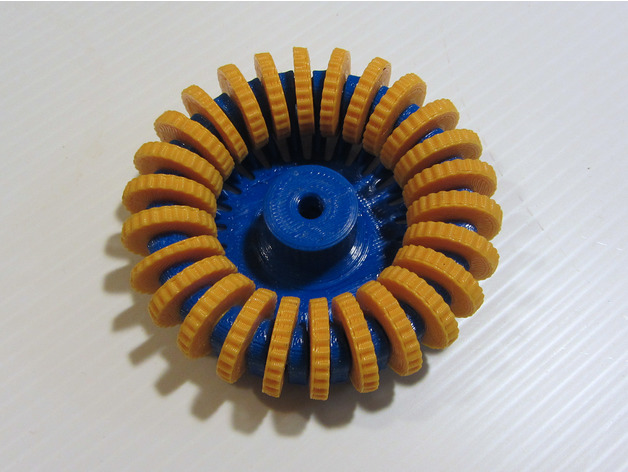
\includegraphics[width=\linewidth]{content/pic/photo/wheel_rings.jpg}
            \column{0.33\textwidth}
                \centering
                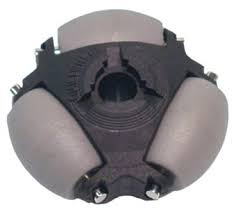
\includegraphics[width=\linewidth]{content/pic/photo/wheel_big_rollers.jpeg}
            \column{0.33\textwidth}
                \centering
                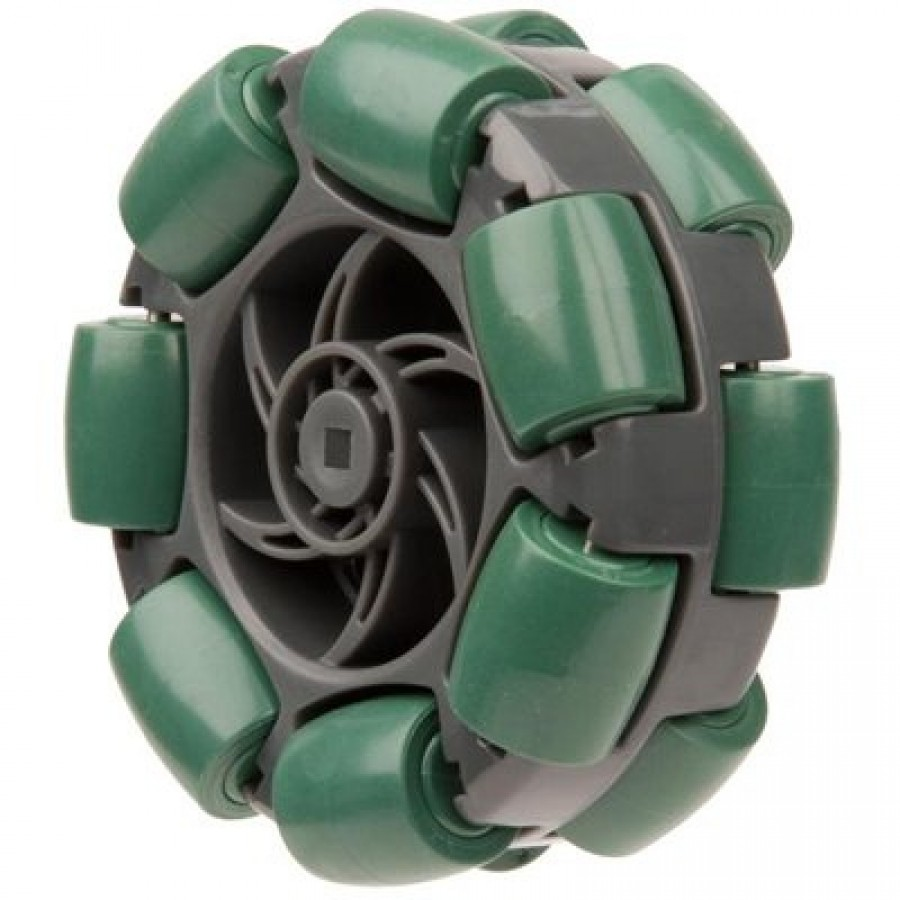
\includegraphics[width=\linewidth]{content/pic/photo/wheel_two_rows.jpg}
        \end{columns}
    \end{figure}
    \vspace{-10pt}
    \begin{figure}[H]
        \centering
        \begin{columns}
            \column{0.45\textwidth}
                \centering
                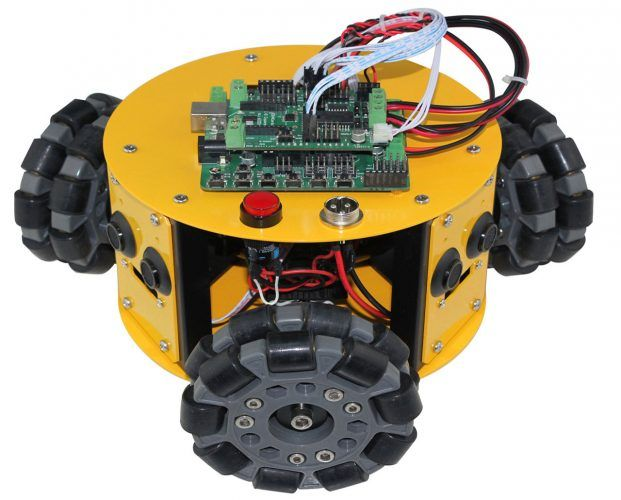
\includegraphics[width=\linewidth]{content/pic/photo/vehicle_three_two_row.jpg}
            \column{0.45\textwidth}
                \centering
                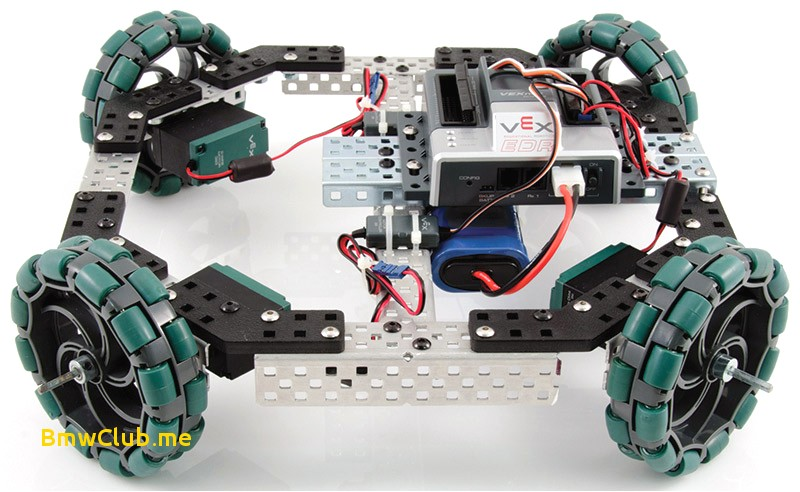
\includegraphics[width=\linewidth]{content/pic/photo/vehicle_four_two_row.jpg}
        \end{columns}
    \end{figure}
\end{frame}

\begin{frame}{Об омни-колесах}{Оси роликов под углом к плоскости колеса (Mecanum)}
    \vspace{10pt}
    \begin{figure}[H]
        \centering
        \begin{columns}
            \column{0.66\textwidth}
                \centering
                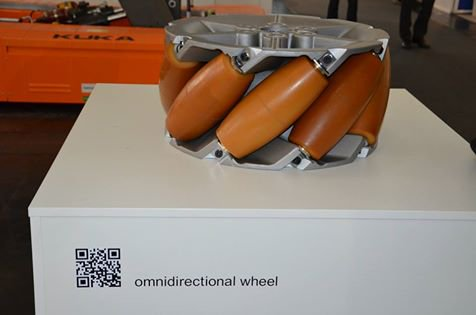
\includegraphics[width=\linewidth]{content/pic/photo/wheel_mecanum.jpg}
        \end{columns}
    \end{figure}
    \vspace{-55pt}
    \begin{figure}[H]
        \centering
        \begin{columns}
            \column{0.85\textwidth}
                \centering
                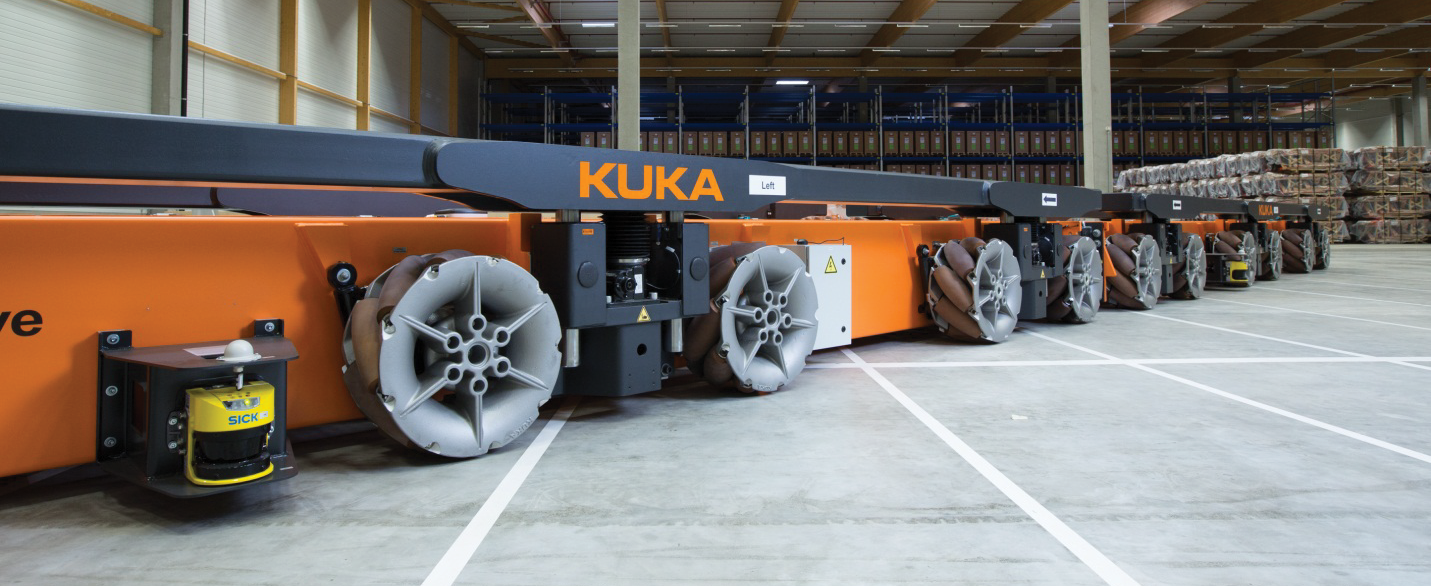
\includegraphics[width=\linewidth]{content/pic/photo/vehicle_kuka.png}
        \end{columns}
    \end{figure}
\end{frame}

\begin{frame}
  \tableofcontents
  % You might wish to add the option [pausesections]
\end{frame}

\section{1. Уравнения движения экипажа по абсолютно шероховатой плоскости с учетом инерции роликов}

\subsection{Постановка задачи}

\begin{frame}{Постановка задачи}{Рисунки}
    \begin{figure}
        \centering
        % \flushleft
        \minipage{0.6\textwidth}
            \asyinclude{content/pic/asy/pic_cart.asy}
            \caption{Экипаж}
        \endminipage
        % \flushright
        \minipage{0.4\textwidth}
            \asyinclude{content/pic/asy/pic_wheel.asy}
            \caption{Колесо}
        \endminipage
    \end{figure}
\end{frame}

\begin{frame}{Постановка задачи}{Тела, связи, степени свободы}
  \begin{itemize}
  \item {
    Экипаж состоит из платформы, $N$ колес и $n$ роликов,\\
    количество твердых тел:
    $$1 + N(n+1)$$
  }
  \item{
    Оси и центры колес и роликов неподвижны относительно\\
    платформы и колес соответственно
  }
  \item {
    Скорость точек контакта равна нулю:
    $$\vec{v}_{C_i} = 0, i = 1\dots N$$
  }
  \item{
    Количество степеней свободы:
    $$3 + N(n-1)$$
  }

  \end{itemize}
\end{frame}

\begin{frame}{Постановка задачи}{Координаты, псевдоскорости, связи}
  \begin{itemize}
  \item {
    Обобщенные координаты: \\
    $q = (x, y, \theta, \chi_i, \phi_k, \phi_s),$ где $i,k = 1\dots N$, $s$ -- ролики вне контакта.
  }
  \item{
    Псевдоскорости:\\
    $\nu = (\nu_1, \nu_2, \nu_3, \nu_s), \vec{v}_S = R\nu_1\vec{e}_\xi + R\nu_2\vec{e}_\eta, \nu_3 = \Lambda\dot{\theta}, \nu_s = \dot{\phi}_s$
  }
  \item {
    Связи:
	$$ \dot{x} = R \nu_1\cos\theta-R\nu_2\sin\theta, \hspace{15pt} \dot{y} = R\nu_1\sin\theta+R\nu_2\cos\theta,$$
	$$\dot{\theta} = \frac{\nu_3}{\Lambda}, \hspace{15pt} \dot{\chi}_i = \frac{R}{l}(\nu_1\sin\alpha_i - \nu_2\cos\alpha_i - \frac{\nu_3}{\Lambda}), $$
	$$ \dot{\phi_k} = \frac{R}{l\cos\chi_k-r}(\nu_1\cos\alpha_k + \nu_2\sin\alpha_k), \hspace{15pt} \dot{\phi}_s = \nu_s $$
  }

  \end{itemize}
\end{frame}

\begin{frame}{Кинетическая энергия и лагранжиан}
  \begin{itemize}
  \item {
    Присутствует слагаемое, пропорциональное $B$ -- моменту инерции ролика относительно его оси собственного вращения:
    $$ 2T = 2L = M\vec{v}_S^2 + I_S\dot{\theta}^2 + J\sum_i\dot{\chi}_i^2 + $$
    $$ + \alert{B\sum_{i,j}(\dot{\phi}_{ij}^2 + 2\dot{\theta}\sin(\kappa_j + \chi_i)\dot{\phi}_{ij})}, $$
    $$ M = \mathring{M} + Nnm $$
    $$ I_S = \mathring{I_S} + N\cdot n(\frac{A+B}{2} + mR^2 + \frac{mr^2}{2}), $$
    $$ J = \mathring{J} + n(A + mr^2) $$
  }

  \end{itemize}
\end{frame}

\begin{frame}{Кинетическая энергия и лагранжиан}
  \begin{itemize}
  \item {
    С учетом связей:
    $$ 2L^{*} = \mathring{\nu}^T \mathring{V}^T \mathring{M} \mathring{V} \mathring{\nu} + $$
    $$ + \alert{B}\sum_{i}(
    	\frac{(\nu_2\sin\alpha_i+\nu_1\cos\alpha_i)^2R^2}
    	{\rho_i^2} + $$
    $$ +
    	\frac{2R\nu_3(\nu_2\sin\alpha_i+\nu_1\cos\alpha_i)\sin\chi_i}
    	{\rho_i\Lambda}
    ) $$
    $$ +
    \alert{B}\sum_{i,j}(
    	\frac{2\nu_3\nu_{ni+j}\sin(\kappa_j+\chi_i)}
    	{\Lambda}
    	+
    	\nu_{ni+j}^2
    )
    $$
    где $ \frac{1}{2}\mathring{\nu}^T \mathring{V}^T \mathring{M} \mathring{V} \mathring{\nu} $ -- лагранжиан системы без роликов, $\rho_i = l\cos\chi_i - r$
  }

  \end{itemize}
\end{frame}

\begin{frame}{Кинетическая энергия и лагранжиан}{Матрицы кинетической энергии и связей для системы без роликов}
    $$ \mathring{M} = diag(M, M, I_S, J...J), $$
    $$ \mathring{V} = \begin{bmatrix}
        R\cos\theta & -R\sin\theta & 0 \\
        R\sin\theta & R\cos\theta  & 0 \\
        0           & 0            & \frac{1}{\Lambda} \\
        \frac{R}{l}\sin\alpha_i & -\frac{R}{l}\cos\alpha_i & -\frac{R}{l\Lambda} \\
    \end{bmatrix} $$
\end{frame}

\subsection{Уравнения движения в форме Я.В. Татаринова}

\begin{frame}{Структура уравнений}{Отличие от случая без роликов}
  \begin{itemize}
  \item {
    Уравнения Я.В. Татаринова:
    \begin{equation}\label{Tatarinov}
    \frac{d}{dt}\frac{\partial L^{*}}{\partial \nu_\alpha}  + \{P_\alpha, L^{*}\} = \{P_\alpha, \nu_\mu P_\mu\},
    \end{equation}
    $$ \nu_\mu P_\mu = \dot{q_i} p_i, \hspace{10pt} p_i = \frac{\partial L}{\partial \dot{q}_i} $$
  }
  \item {
    Лагранжиан и ``импульсы'' отличаются аддитивными членами:
    $$ L^{*} = \mathring{L}^{*} + BL^{*}_\Delta(\nu, \chi) $$
    $$ P_\alpha = \mathring{P_\alpha}(\theta, p_x, p_y, p_\chi) + P_\Delta(p_{\phi_i}, \chi) $$
  }

  \end{itemize}
\end{frame}

\begin{frame}{Структура уравнений}{Матрица лагранжиана}    
Лагранжиан с учетом связей имеет вид:
$$ 2L^{*}  = \vec{\nu}^\mathrm{T} V^\mathrm{T}\M V\vec{\nu} = \vec{\nu}^\mathrm{T} \M^*(\chi_i)\vec{\nu} $$
Структура симметричной матрицы $\M^*$ следующая:
$$
\M^* = \begin{bmatrix}
        \left(\begin{matrix}&&\\&m^*_{ij}&\\&&\end{matrix}\right)_{3\times3} \quad & \left(\begin{matrix} 0&\ldots& 0 \\ 0&\ldots&0 \\ B\Lambda^{-1}\sin\chi_{12}&\ldots& B\Lambda^{-1}\sin\chi_{nN} \end{matrix}\right) \\[25pt]
        *          & \begin{matrix} B & & \\ & \ddots & \\ & & B \end{matrix} \\
    \end{bmatrix}
$$
\end{frame}

\begin{frame}{Структура уравнений}{Слагаемые для свободных роликов}    
Первое слагаемое (\ref{Tatarinov}) получается дифференцированием лагранжиана и подстановкой связей (ниже $\M^*_i = \ddfrac{\partial \M^*}{\partial \chi_i}$):
\begin{equation*}
    \frac{d}{dt}\frac{\partial L^{*}}{\partial \nu_\alpha} = \frac{d}{dt}(\M^*(\chi)\vec{\nu}_\alpha) = 
    \M^*(\chi_i)\dot{\vec{\nu}_\alpha} +
    \left(\sum_{i=1}^{N}\M^*_i(V\nu)_{3+i}\vec{\nu}\right)_\alpha,
\end{equation*}
Cлагаемые, соответствующие свободным роликам:
\begin{equation*}
    \frac{\cos\chi_{ij} \nu_3 B \left( -\ddfrac{\nu_3 R}{l \Lambda}-\ddfrac{\cos\alpha_i \nu_2 R}{l}+\ddfrac{\sin\alpha_i \nu_1 R}{l}\right) }{\Lambda} = \frac{B}{\Lambda}\cos\chi_{ij}(\dot{\chi_i})^*\nu_3.
\end{equation*}
\end{frame}

\begin{frame}{Структура уравнений}{Детали}
Формальные импульсы $P_\alpha$ и скобки Пуассона $L^{*}$ с ними:
\begin{equation*}\label{P}
    \begin{array}{rcl}
        P_1 & = & R\bigg(p_x\cos\theta + p_y\sin\theta + \sum\limits_{i}\bigg(\ddfrac{\sin\alpha_ip_{\chi_i}}{l} +  \ddfrac{\cos\alpha_ip_{\phi_{i1}}}{\rho_i}\bigg)\bigg),\vsp
        P_2 & = & R\bigg(-p_x\sin\theta + p_y\cos\theta + \sum\limits_{i}\bigg(-\ddfrac{\cos\alpha_ip_{\chi_i}}{l} +  \ddfrac{\sin\alpha_ip_{\phi_{i1}}}{\rho_i}\bigg)\bigg),\vsp
        P_3 & = & \ddfrac{1}{\Lambda}\bigg(p_\theta - \sum\limits_{i}\ddfrac{R}{l}p_{\chi_i}\bigg), \quad P_s p_{\phi_s},
    \end{array}
\end{equation*}

$$
\{P_1, L^*\} = -\frac{\partial P_1}{\partial p_{\chi_i}}\frac{\partial L^*}{\partial \chi_i} = -\frac{R}{2l}\vec{\nu}^\mathrm{T}\sin\alpha_i\M^*_i\vec{\nu},
$$
$$
\{P_2, L^*\} = \frac{R}{2l}\vec{\nu}^\mathrm{T}\cos\alpha_i\M^*_i\vec{\nu},\  
\{P_3, L^*\} = \frac{R}{2l\Lambda}\vec{\nu}^\mathrm{T}\M^*_i\vec{\nu},\quad \{P_s,L^*\} = 0,
$$

Cуммы $\{P_\alpha, \nu_\mu P_\mu\} \neq 0$ лишь для первых трех уравнений.
\end{frame}

\begin{frame}{Уравнения движения}{в форме Я.В. Татаринова}
    \begin{columns}
        \hspace{-4pt}
        \begin{column}{0.4\textwidth}
            \vspace{-40pt}
            \begin{equation*}
            \qquad
            \frac{d}{dt}\frac{\partial L^{*}}{\partial \nu_\alpha}  + \{P_\alpha, L^{*}\} = \{P_\alpha, \nu_\mu P_\mu\}
            \end{equation*}
            $$
            \qquad
            \nu_\mu P_\mu = \dot{q_i} p_i, \hspace{10pt} p_i = \frac{\partial L}{\partial \dot{q}_i}
            $$
            \vspace{20pt}
            $$
            \quad
            L^{*}  = \ddfrac{1}{2}\vec{\nu}^\mathrm{T} \cstr^\mathrm{T}\mke \cstr\vec{\nu} = \ddfrac{1}{2}\vec{\nu}^\mathrm{T} \mke^*(\chi_i)\vec{\nu}
            $$
        \end{column}
        \hspace{46pt}
        \begin{column}{0.6\textwidth}
            \vspace{-20pt}
            \begin{eqnarray*}
                \mke & = &
                    \begin{bmatrix}
                        \widetilde{\mke}_{11} & O_{3 \times N}  & \widetilde{\mke}_{13} \\
                                            & JE_{N \times N} & O_{N \times Nn}     \\
                        \star               &                 & BE_{Nn \times Nn}   \\
                    \end{bmatrix} \\
                \widetilde{\mke}_{11} & = & \text{diag}(M, M, I_S) \\
                \widetilde{\mke}_{13} & = &
                    \begin{bmatrix}
                        0                      & \cdots & 0                      \\
                        0                      & \cdots & 0                      \\
                        B\sin\chi_{11}         & \cdots & B\sin\chi_{Nn}         \\
                    \end{bmatrix} \\
                \mathring{V} & = &
                    \begin{bmatrix}
                        R\cos\theta & -R\sin\theta & 0 \\
                        R\sin\theta & R\cos\theta  & 0 \\
                        0           & 0            & \frac{1}{\Lambda} \\
                        \frac{R}{l}\sin\alpha_i & -\frac{R}{l}\cos\alpha_i & -\frac{R}{l\Lambda} \\
                    \end{bmatrix}
            \end{eqnarray*}
        \end{column}
    \end{columns}
\end{frame}

\subsection{Свойства и сравнение с безынерционной моделью}

\begin{frame}{Структура уравнений}{Новые слагаемые ($\Prhs_\alpha$ и $\M^*_i$ зависят от $\chi$)}
\vspace{-15pt}
\begin{eqnarray*}\label{eq:full_system}
\M^*\dot{\vec{\nu}} & = & 
\frac{MR^2}{\Lambda}\left(\begin{matrix}
    \nu_2\nu_3\\
    -\nu_1\nu_3\\
    0\\
    0\\
    \vdots
    \\
    0
\end{matrix}\right)
+
\frac{R}{2l}
\vec{\nu}^\mathrm{T}
\left(\begin{matrix}
    -\sin\alpha_i \M^*_i\\
    \cos\alpha_i \M^*_i\\
    \Lambda^{-1}\M^*_i\\
    0\\
    \vdots
    \\
    0
    \end{matrix}
\right)
\vec{\nu}
\\
 & - & BR^2
\vec{\nu}^\mathrm{T}
\left(\begin{matrix}
    \Prhs_1\\
    \Prhs_2\\
    \Prhs_3\\
    0\\
    \vdots
    \\
    0
\end{matrix}\right)
\vec{\nu}
\ - \
B\left(\begin{matrix}
    *\\
    *\\
    *\\
    \cos\chi_{12}\ddfrac{\nu_3}{\Lambda}\dot{\chi_1^*}\\
    \vdots
    \\
    \cos\chi_{Nn}\ddfrac{\nu_3}{\Lambda}\dot{\chi_N^*}
\end{matrix}\right)
\end{eqnarray*}
\end{frame}

\begin{frame}{Структура уравнений}{Свойства}    
\begin{enumerate}
    \item Интеграл энергии \quad $\frac{1}{2}\vec{\nu}^\mathrm{T}\M^*(\chi_i)\vec{\nu} = h = \mathrm{const}$\\
    (связи автономны, идеальны, силы консервативны)
    \item $\nu_1 = \nu_2 = \nu_3 = 0 \quad \implies \quad \nu_s = \mathrm{const}$
    \item $B = 0 \ \implies$ уравнения как в безынерционной модели.
    \item Интеграл $m_{33}^*\nu_3 = \mathrm{const}$ разрушается при $B \neq 0$. \ $\dot{\nu_3} \textprop B$.
    \item Первые интегралы:
    $$\nu_s + \ddfrac{1}{\Lambda}\sin\chi_{ij}\nu_3 = const.$$
    Вращение $\nu_1(0) = 0, \nu_2(0) = 0, \nu3(0) \neq 0$ неравномерно.
    \item Замена псевдоскоростей $\vec{\nu} \rightarrow \lambda\vec{\nu}, \lambda \neq 0$ эквивалентна замене времени $t \rightarrow \lambda t$.
\end{enumerate}
\end{frame}


\section{2. Смена ролика в контакте колеса и опорной плоскости}

\begin{frame}{Смена ролика}
    \textcolor{Periwinkle}{(1) Уравнения вырождаются на стыках роликов:}\\
    \textit{разрыв 2ого рода в правой части из-за выражений $(l\cos\chi_i-r)$ в знаменателе.} \\
    Пусть переход на следующий ролик будет раньше стыка.
    \begin{figure}
        \centering
        \asyinclude{content/pic/asy/pic_overlap.asy}
        \caption{Ролики перекрываются}
    \end{figure}
\end{frame}

\begin{frame}{Смена ролика}
    \textcolor{Periwinkle}{(2) Ролики входят и выходят из состояния контакта при $t = t^*$.}\\
    Происходит мгновенное снятие связи с одного ролика и наложение связи на другой.\\
    Пусть:
    \begin{itemize}
        \item $\Delta t << 1$, $\quad \Delta \q \sim \nu\Delta t << 1$, $\quad \Delta \nu < \infty$,
        \item в точках контакта: $\quad \mathbf{R} = \mathbf{N} + \mathbf{F}$, $\quad \mathbf{M} = 0 $,
        \item трения в осях нет,
        \item к моменту окончания удара $t^*+\Delta t$ уравнения связей выполнены (\enspace $\dqposle = \cstr(\q)\nuposle \ $), т.е. за время $\Delta t$ проскальзывание вошедшего в контакт ролика закончилось
    \end{itemize}
\end{frame}

\subsection{Основное уравнение теории удара}

\begin{frame}{Основное уравнение теории удара}{Линейная система алгебраических уравнений на реакции и скорости после удара}
    \begin{columns}
        \hspace{15pt}
        \begin{column}{0.35\textwidth}
            \vspace{-10pt}
            $$ \eqDeltaqQ $$
            $$ \J\dqposle = 0, \quad \Q^T\delta\qposle = 0 $$
            $$ \eqQJtF, \enspace \eqqnu, \enspace \J\cstr = 0 $$
            $$ \eqMVnuJtF $$
            $$ \eqMVnuJtFmatres $$
            \begin{eqnarray*}
                \dim \mke \cstr & = & \dim \q \times \dim \nuvec \\
                \dim \J^T & = & \dim \q \times \dim \F \\
                \dim \q & = & 3 + N(n + 1) \\
                \dim \nuvec & = & 3 + N(n - 1) \\
                \dim \F & = & 2N
            \end{eqnarray*}
        \end{column}
        \hspace{55pt}
        \begin{column}{0.65\textwidth}
            \begin{figure}
                % \centering
                \hspace{-55pt}
                \asyinclude{content/pic/asy/pic_react.asy}
                \caption{Касательные реакции в точках контакта}
            \end{figure}
        \end{column}
    \end{columns}
\end{frame}

\begin{frame}{Основное уравнение теории удара}{Ударные обобщенные импульсы и реакции}
    \vspace{-5pt}
    $$ \eqQ $$
    \vspace{-15pt}
    \begin{eqnarray*}
    \eqQiOne \\
    \eqQiTwo \\
    \eqQiTheta \\
    \eqQChii \\
    \eqQPhii \\
    \eqQs
    \end{eqnarray*}
\end{frame}

\begin{frame}{Независимое нахождение обобщенных скоростей}
    \begin{columns}
        \hspace{15pt}
        \begin{column}{0.35\textwidth}
            $$ \dqposle = \dqdo -\ \deltadq = \mathbf{V}\nuposle \in \subspace $$
            \begin{eqnarray*}
                0 & = & \dotp{\deltadq}{\mke\cstr} \\
                  & = & \dotp{\cstr\nuposle - \dqdo}{\mke\cstr} \\
                  & = & \dotp{\mke\cstr\nuposle - \mke\dqdo}{\cstr} \\
                  & = & \cstr^T\mke\cstr\nuposle - \cstr^T\mke\dqdo
            \end{eqnarray*}
            \vspace{0.35pt}
            $$ \eqnuposleproj $$
        \end{column}
        \hspace{55pt}
        \begin{column}{0.65\textwidth}
            \begin{figure}
                % \centering
                \hspace{-65pt}
                \asyinclude{content/pic/asy/pic_project}
                \caption{
                    $\dqposle$ -- проекция $\dqdo$ на $\subspace$,\newline
                    ортогональная в метрике $\mke$
                }
            \end{figure}
        \end{column}
    \end{columns}
\end{frame}

\begin{frame}{Нахождение обобщенных скоростей и ударных реакций}
    
    Основное уравнение удара  \quad \quad \quad \quad $ \eqDeltaqQ $ \\
    Дифференциальные связи  \quad \quad \quad \quad $ \J\dqposle = 0 $ \\
    Условие идеальности связей \quad \quad \quad $ \Q^T\delta\qposle = 0 $ \\

    Система разрешима относительно $\nuFT$
    $$ \eqMVnuJtF $$
    Скорости находятся независимо от сил ($\cstr^T\cdot$)    
    $$ \eqnuposleproj $$
    Скорости находятся независимо от сил ($\J\mke^{-1}\cdot$)    
    $$ \eqFproj $$
    
\end{frame}


\subsection{Изменение энергии}

\begin{frame}{Изменение энергии}{Соответствует теореме Карно}
    $$ \eqTquad, \quad \eqDqVnu $$

    В силу идеальности связей:
    $$ \logicWorkZero $$
    
    Поэтому:
        $$ \eqDeltaT $$
    \begin{eqnarray*}
        2\Delta\ke & = & 2\left(\ke^+ - \ke^-\right) = \dotp{\mke\dqposle}{\dqposle} - \dotp{\mke\dqdo}{\dqdo} \\
        & = & \dotp{\mke\deltadq}{\deltadq} + 2\dotp{\mke\dqdo}{\deltadq} \\
        & = & -\dotp{\mke\deltadq}{\deltadq} + 2\dotp{\mke\dqposle}{\deltadq} = -\dotp{\mke\deltadq}{\deltadq}
    \end{eqnarray*}
\end{frame}

\subsection{Численное решение}

\begin{frame}{Значения параметров}
    \begin{itemize}
        \item радиус колеса $r = 0.05$,
        \item масса колеса $ M_{\text{к}} = 0.15$, 
        \item масса ролика $m_{\text{рол}} = 0.05$, 
        \item радиус платформы $R = 0.15$, 
        \item масса платформы $M_{\text{пл}} = 1$.
    \end{itemize}
\end{frame}

\begin{frame}{Вращение вокруг своей оси ($\nu_{1,2}(0) = 0, \nu_3 = 1$).}
    \begin{figure}[H]
        \centering
        \begin{columns}
            \column{0.33\textwidth}
                \centering
                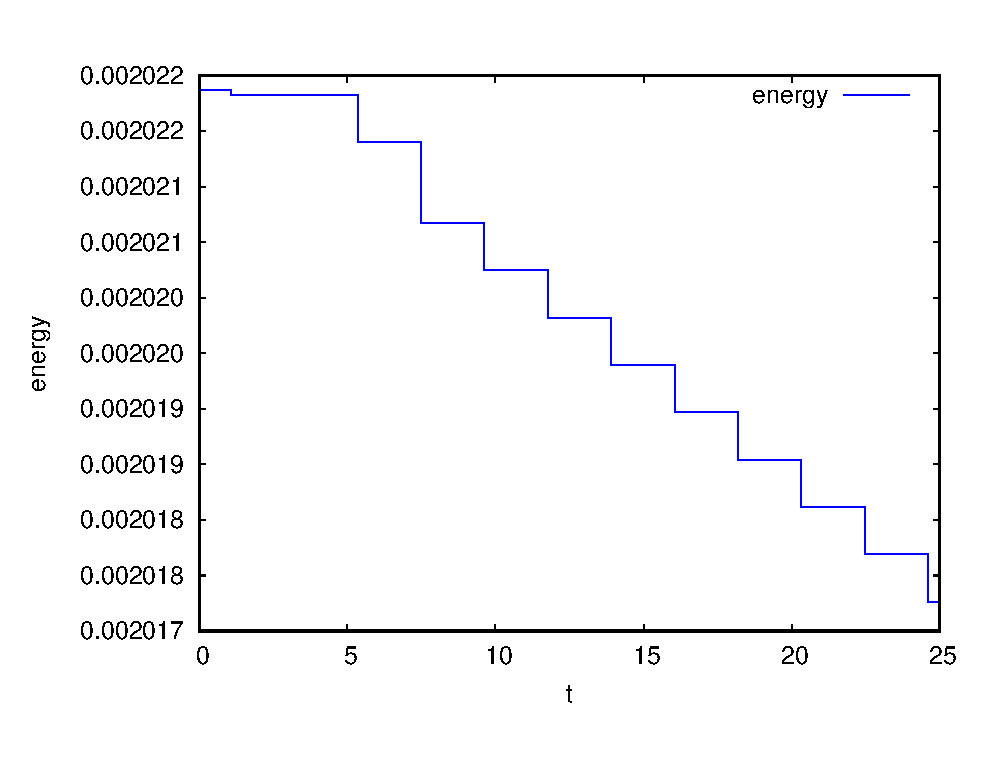
\includegraphics[width=\linewidth]{content/pic/self_rot_25/kin_en.eps}
                \vspace{-15pt}
                \caption{Кинетическая энергия}
            \column{0.33\textwidth}
                \centering
                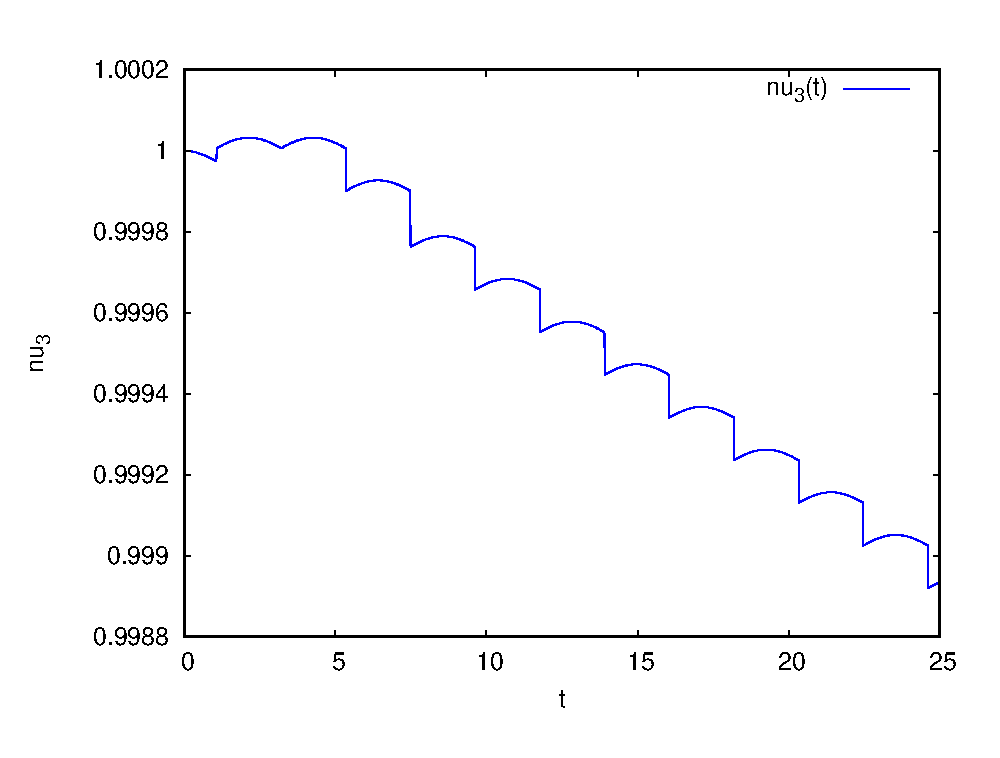
\includegraphics[width=\linewidth]{content/pic/self_rot_25/nu3.eps}
                \vspace{-15pt}
                \caption{Угловая скорость экипажа}
            \column{0.33\textwidth}
                \centering
                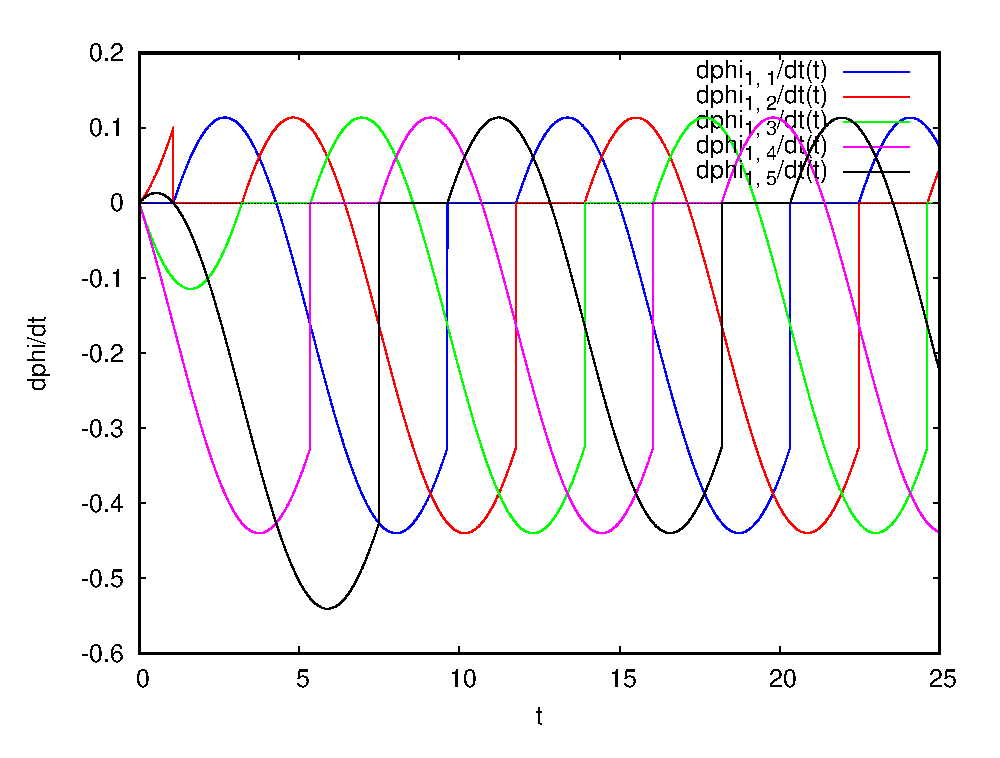
\includegraphics[width=\linewidth]{content/pic/self_rot_25/rol_vel.eps}
                \vspace{-15pt}
                \caption{Угловые скорости роликов}
        \end{columns}
    \end{figure}
    \vspace{-25pt}
    \begin{figure}[H]
        \centering
        \begin{columns}
            \column{0.33\textwidth}
                \centering
                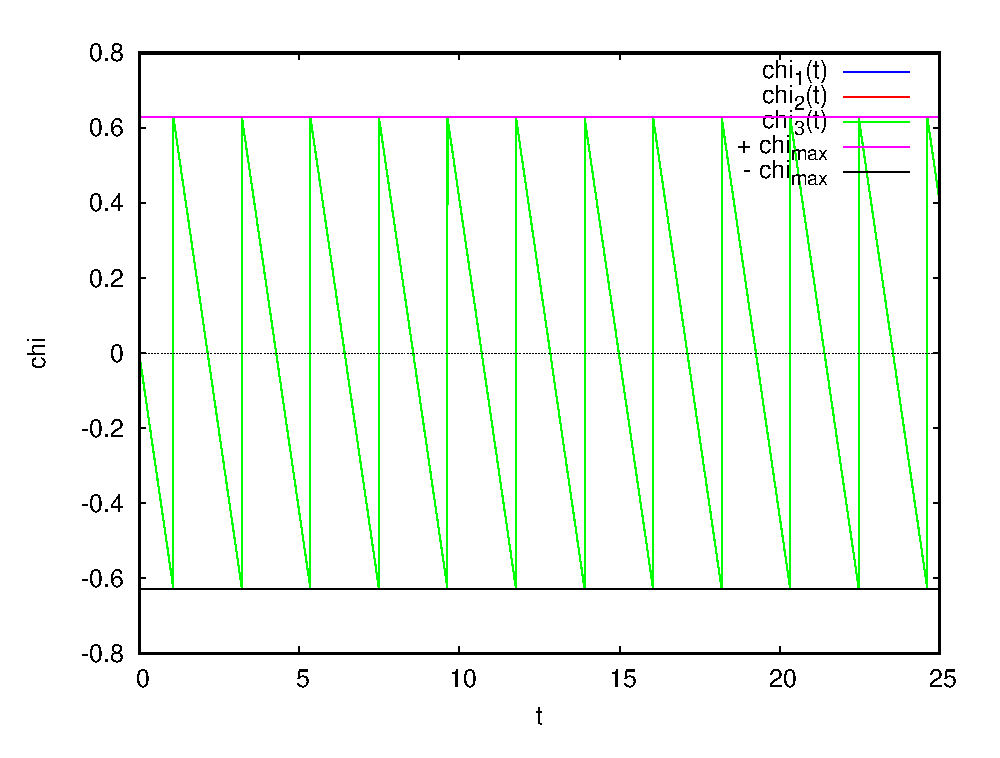
\includegraphics[width=\linewidth]{content/pic/self_rot_25/chi.eps}
                \vspace{-15pt}
                \caption{Углы поворота колес}
            \column{0.33\textwidth}
                \centering
                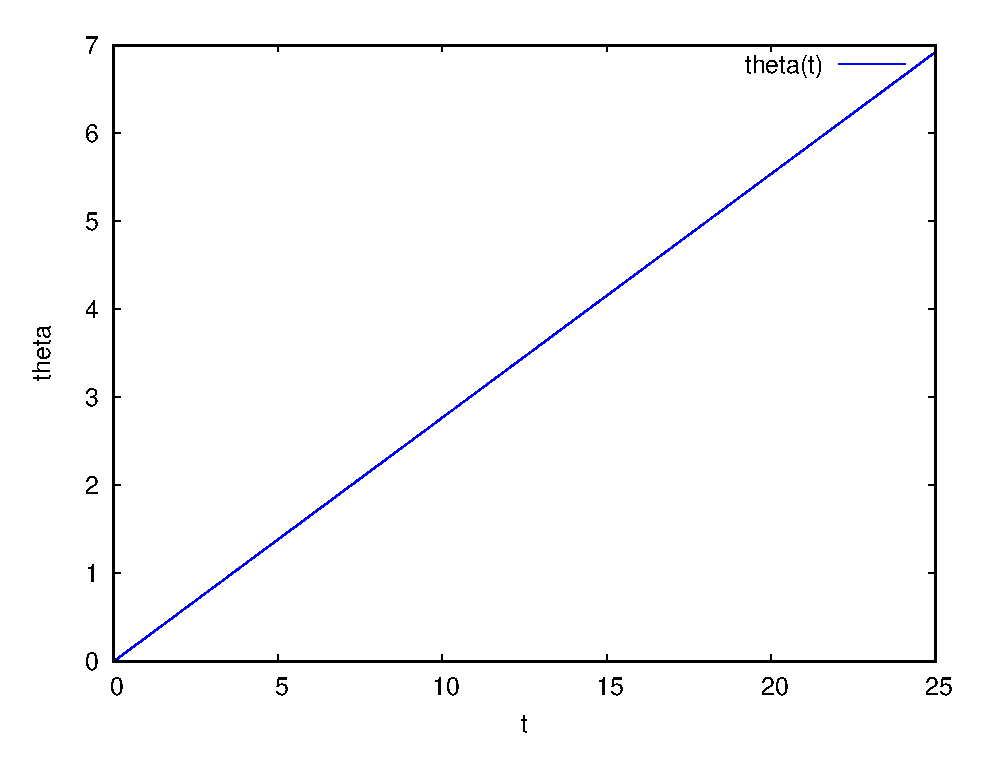
\includegraphics[width=\linewidth]{content/pic/self_rot_25/theta.eps}
                \vspace{-15pt}
                \caption{Угол поворота экипажа}
            \column{0.33\textwidth}
                \centering
                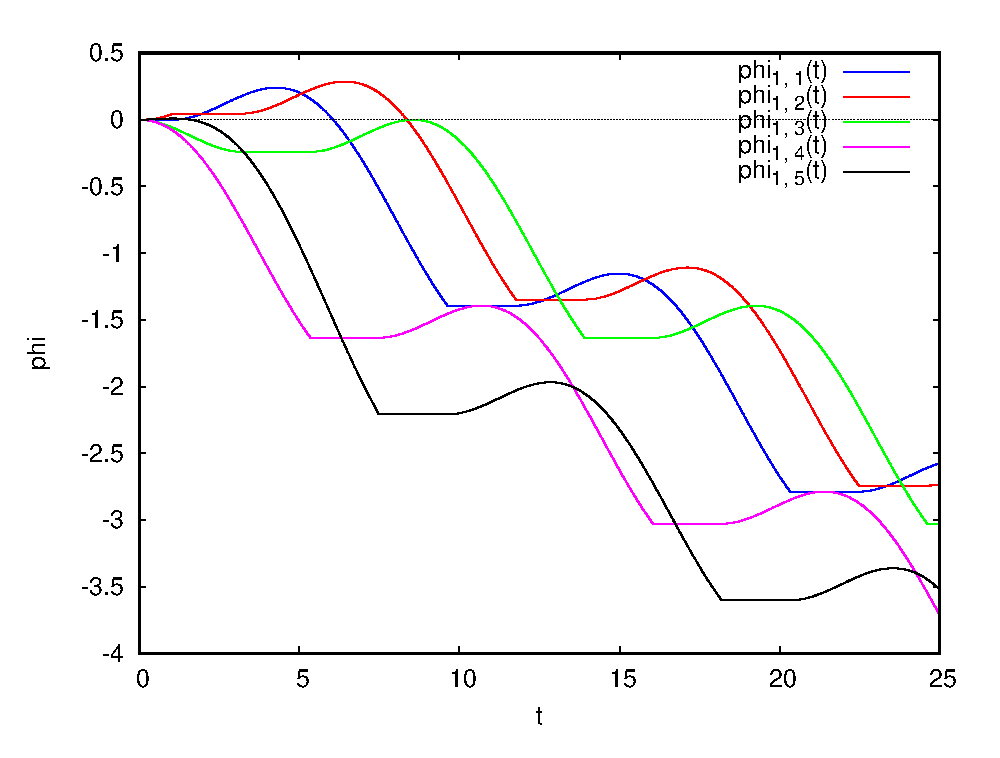
\includegraphics[width=\linewidth]{content/pic/self_rot_25/rol_ang.eps}
                \vspace{-15pt}
                \caption{Углы поворота роликов}
        \end{columns}
    \end{figure}
\end{frame}

\begin{frame}{Движение по прямой ($\nu_1(0) = 1, \nu_{2,3} = 0$).}
    \begin{figure}[H]
        \centering
        \begin{columns}
            \column{0.25\textwidth}
                \centering
                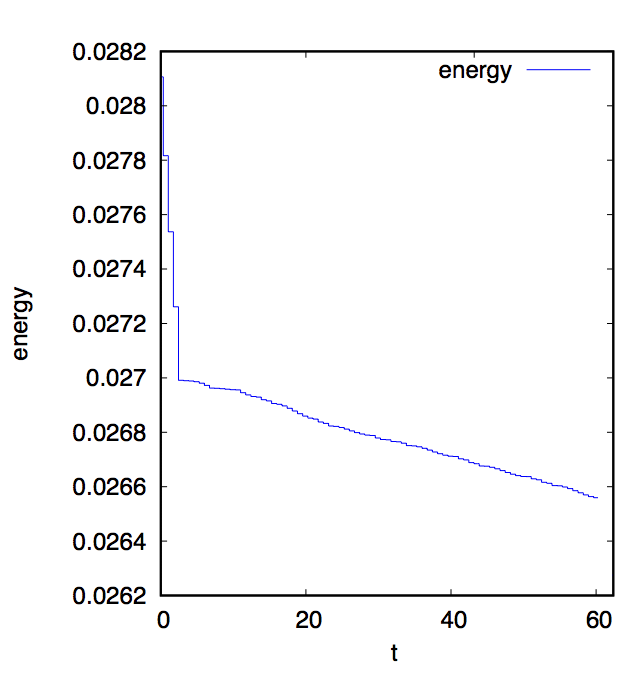
\includegraphics[width=1.1\linewidth]{content/pic/straight_60/kin_en.png}
                \vspace{-15pt}
                \caption{Кинетическая энергия}
            \column{0.37\textwidth}
                \centering
                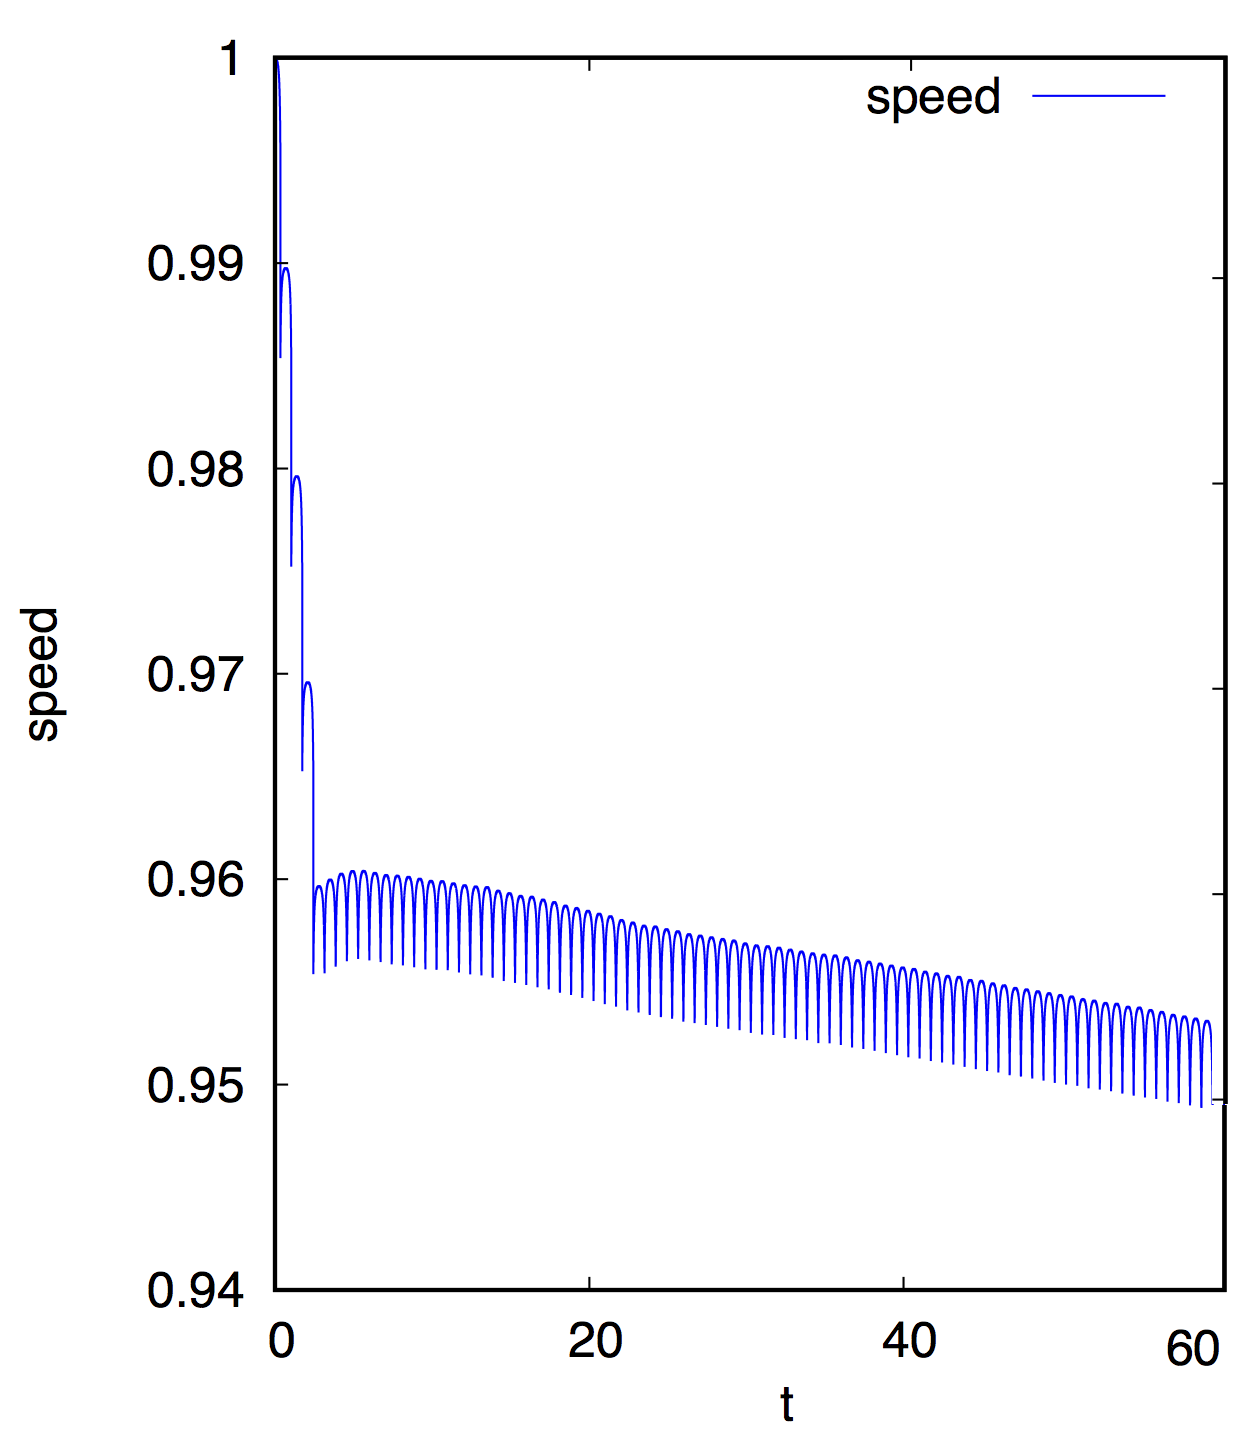
\includegraphics[width=0.8\linewidth]{content/pic/straight_60/v.png}
                \vspace{-15pt}
                \caption{Скорость центра масс}
            \column{0.37\textwidth}
                \centering
                \vspace{2.5pt}
                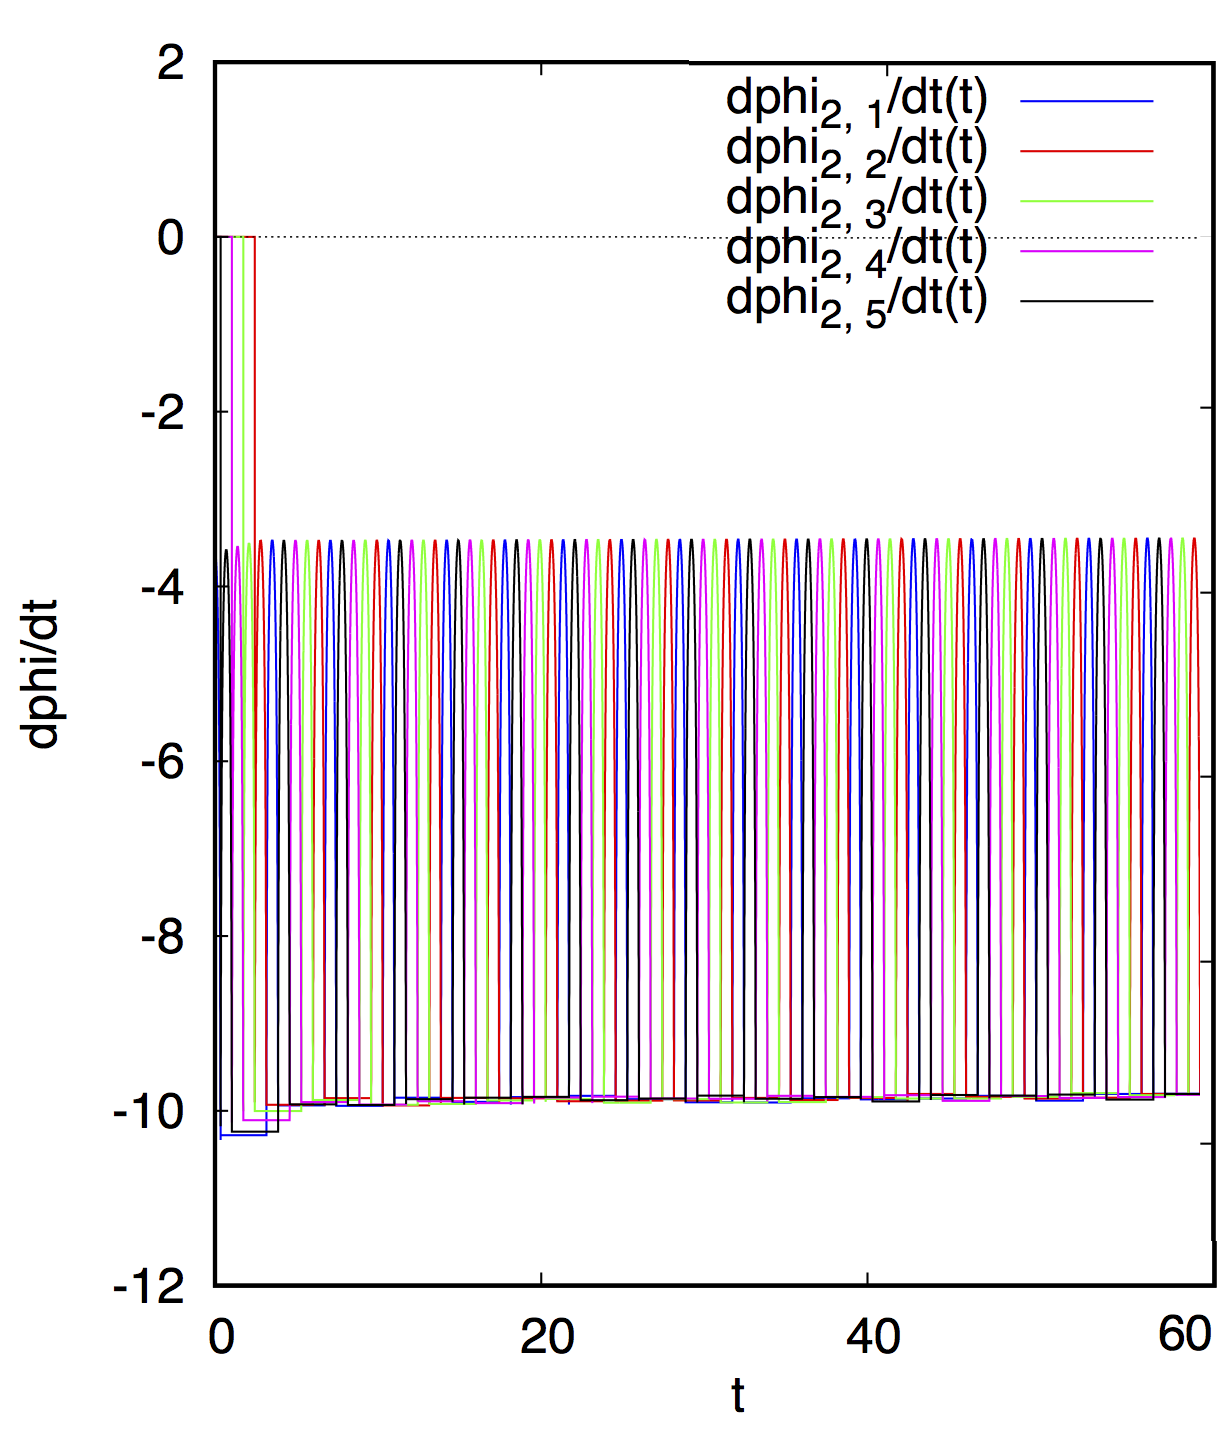
\includegraphics[width=0.8\linewidth]{content/pic/straight_60/nus2.png}
                \vspace{-15pt}
                \caption{$\dot{\mathbf{\phi}}$ на заднем колесе}
        \end{columns}
    \end{figure}
    \vspace{-25pt}
    \begin{figure}[H]
        \centering
        \begin{columns}
            \column{0.33\textwidth}
                \centering
                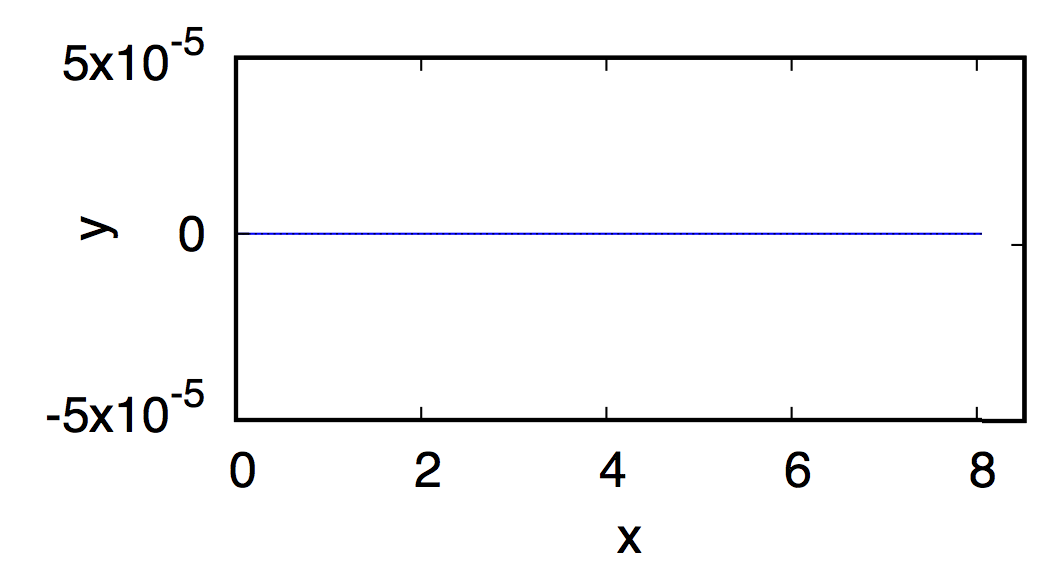
\includegraphics[width=\linewidth]{content/pic/straight_60/traj.png}
                \vspace{-15pt}
                \caption{Траектория}
            \column{0.33\textwidth}
                \centering
                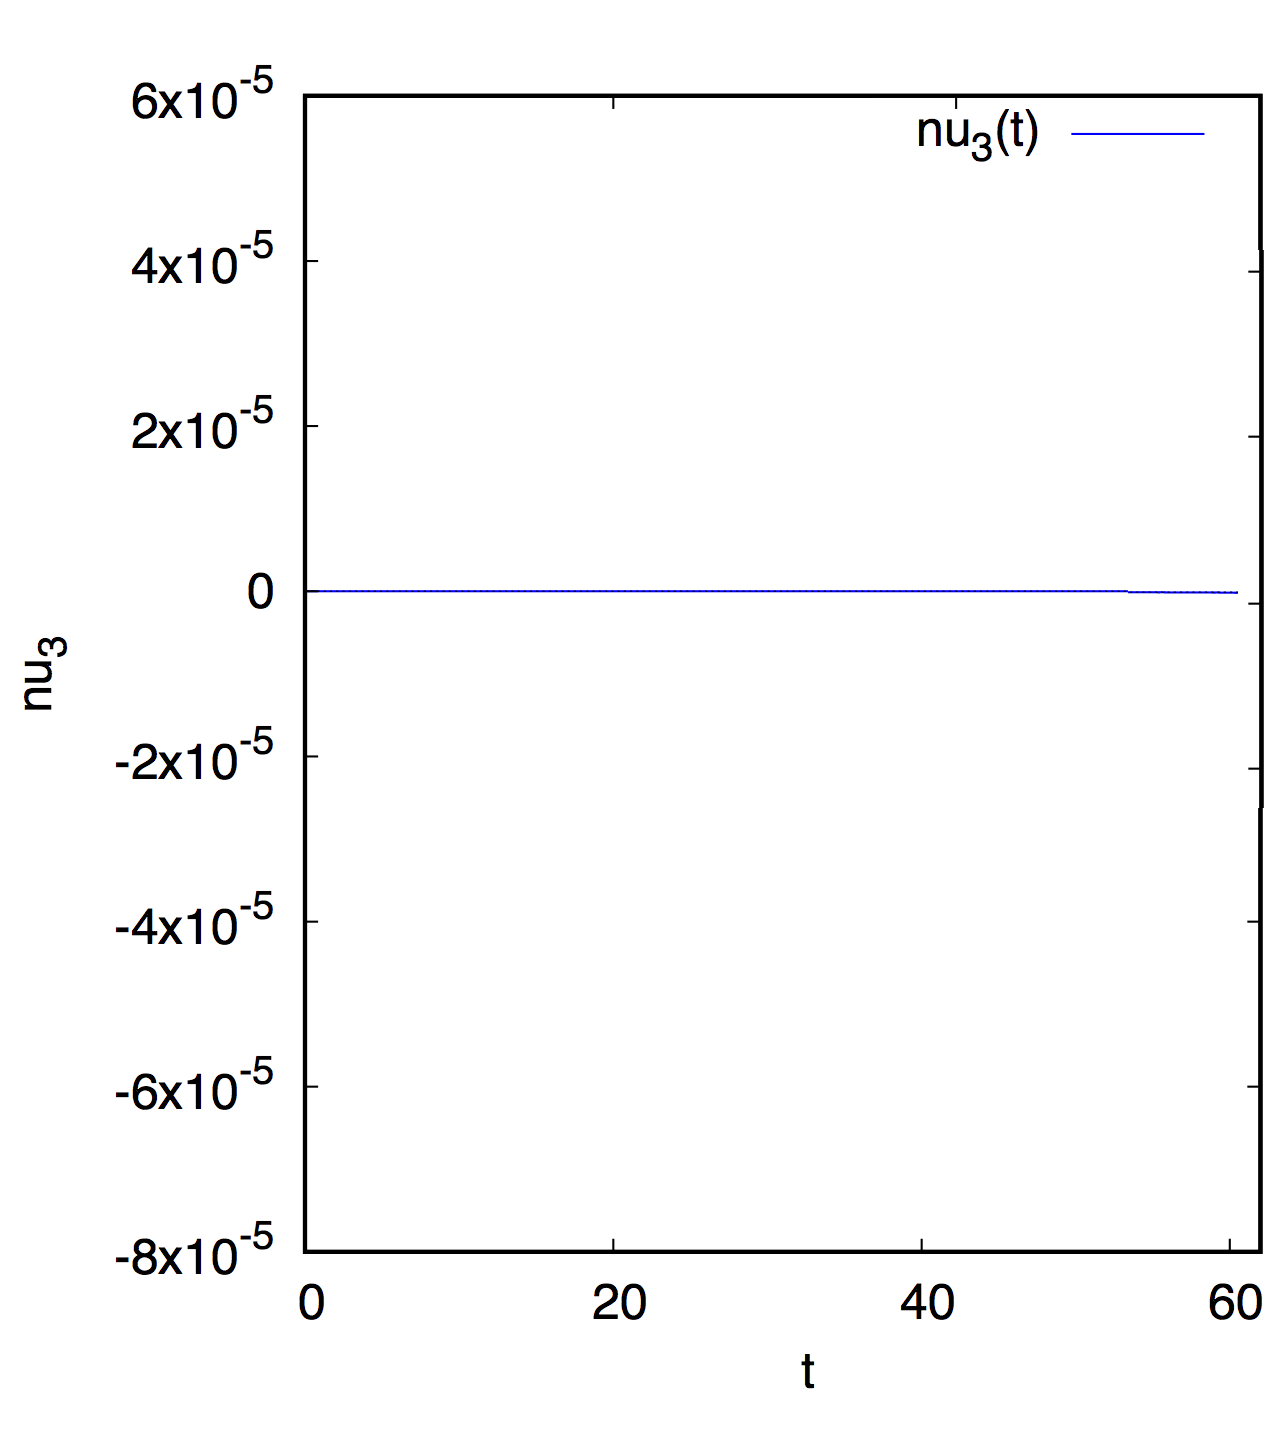
\includegraphics[width=0.8\linewidth]{content/pic/straight_60/nu3.png}
                \vspace{-15pt}
                \caption{Угловая скорость экипажа}
            \column{0.33\textwidth}
                \centering
                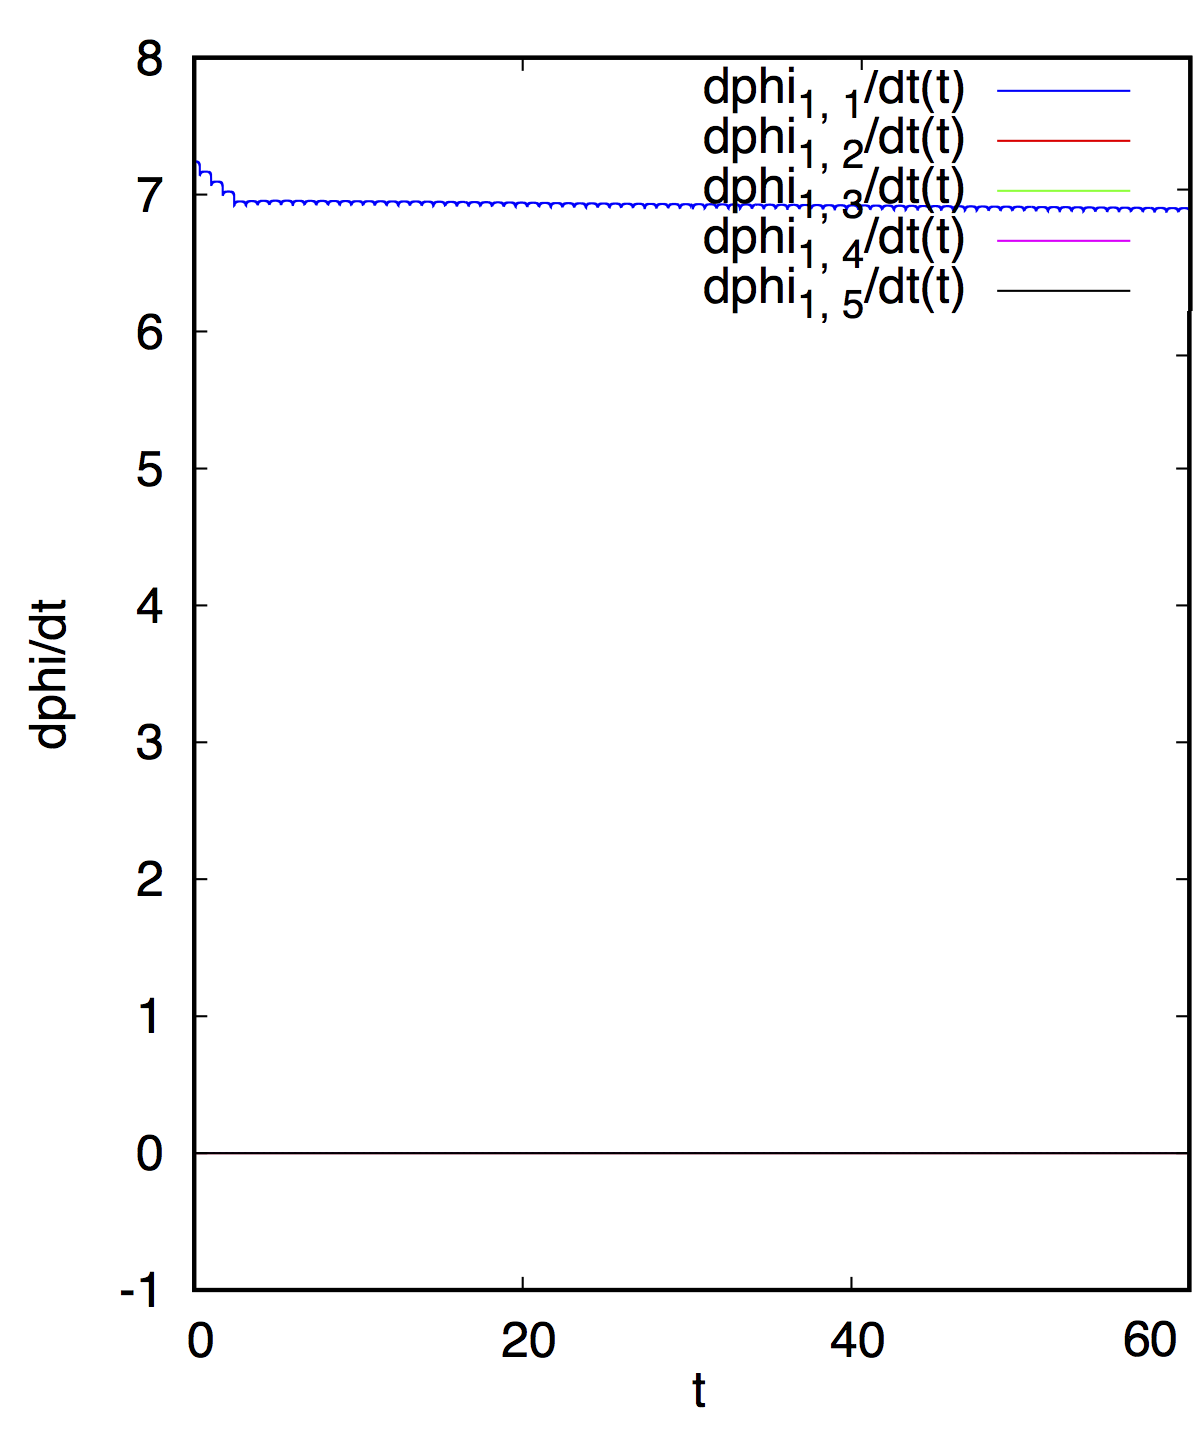
\includegraphics[width=0.8\linewidth]{content/pic/straight_60/nus1.png}
                \vspace{-15pt}
                \caption{$\dot{\mathbf{\phi}}$ на переднем колесе}
        \end{columns}
    \end{figure}
\end{frame}

\begin{frame}{Движение с закруткой ($\nu_1(0) = 1, \nu_2(0) = 0, \nu_3(0) = 1$).}
    \begin{figure}[H]
        \centering
        \begin{columns}
            \column{0.33\textwidth}
                \centering
                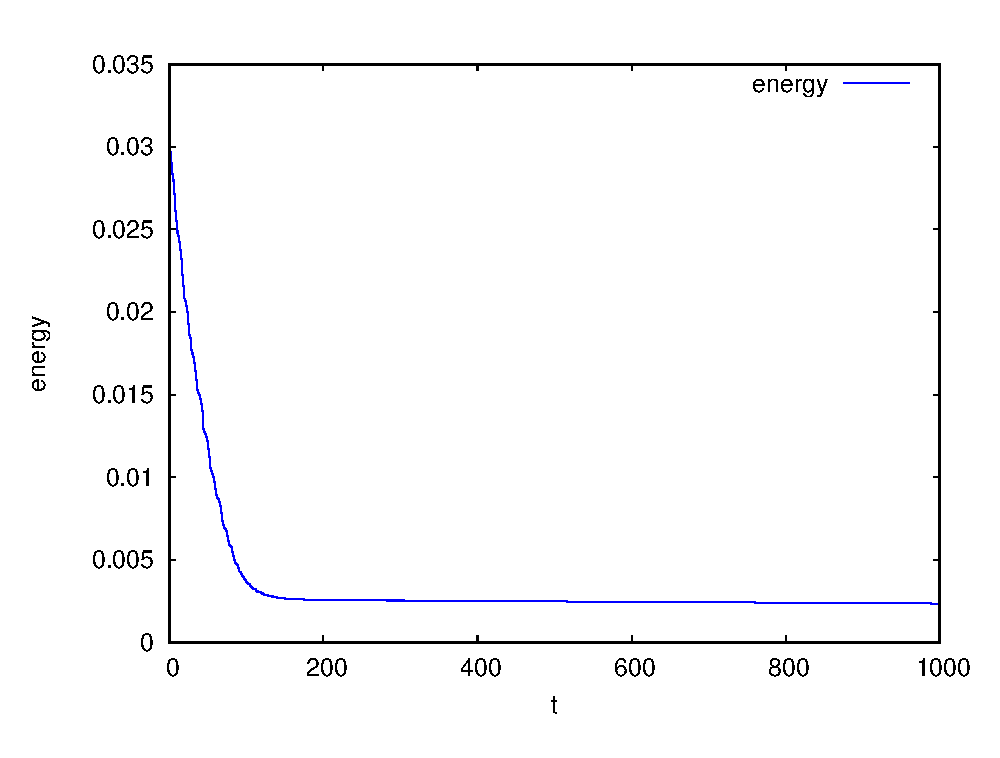
\includegraphics[width=\linewidth]{content/pic/wrench_1000/kin_en.eps}
                \vspace{-15pt}
                \caption{Кинетическая энергия}
            \column{0.33\textwidth}
                \centering
                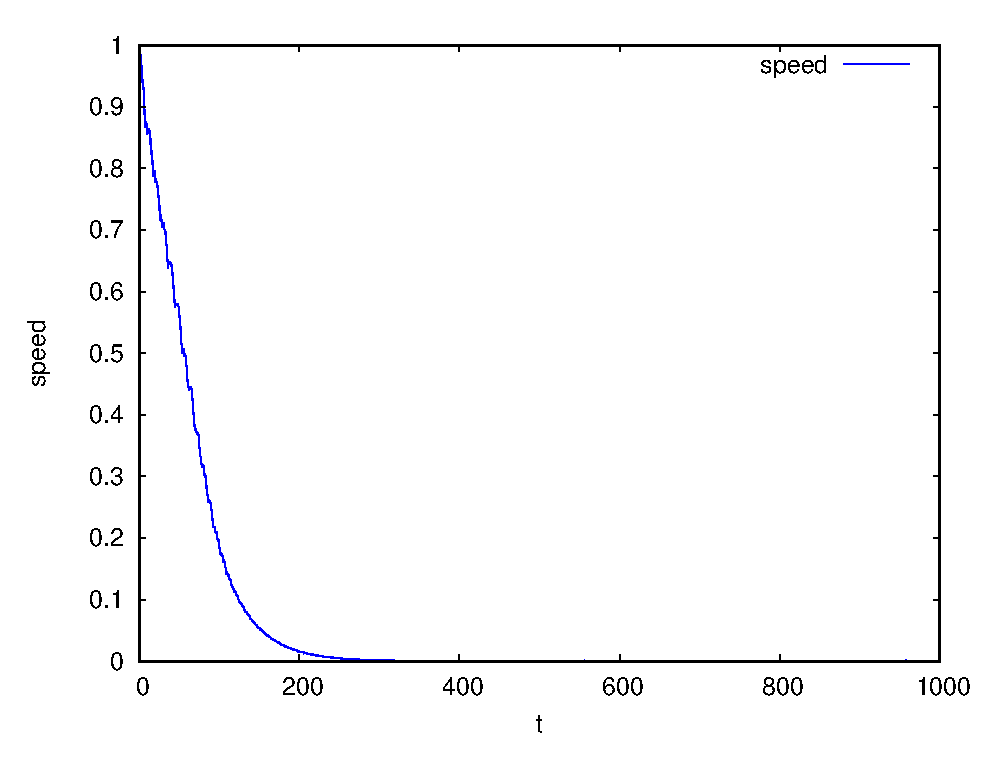
\includegraphics[width=\linewidth]{content/pic/wrench_1000/v.eps}
                \vspace{-15pt}
                \caption{Скорость центра масс}
            \column{0.33\textwidth}
                \centering
                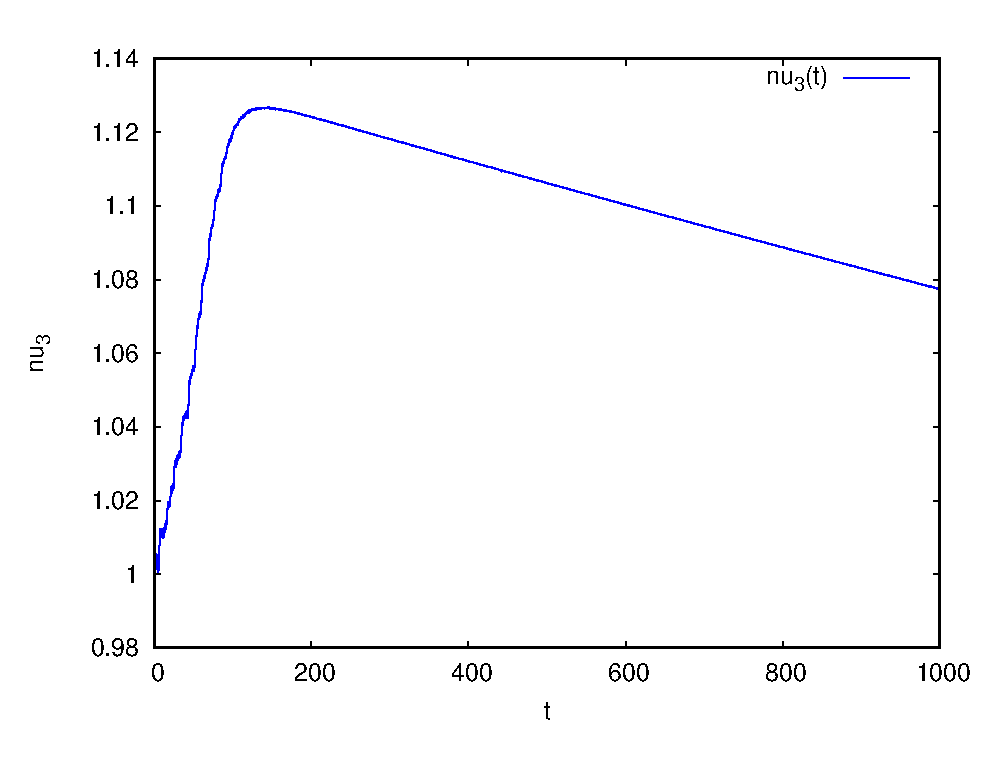
\includegraphics[width=\linewidth]{content/pic/wrench_1000/nu3.eps}
                \vspace{-15pt}
                \caption{Угловая скорость экипажа}
        \end{columns}
    \end{figure}
    \vspace{-25pt}
    \begin{figure}[H]
        \centering
        \begin{columns}
            \column{0.33\textwidth}
                \centering
                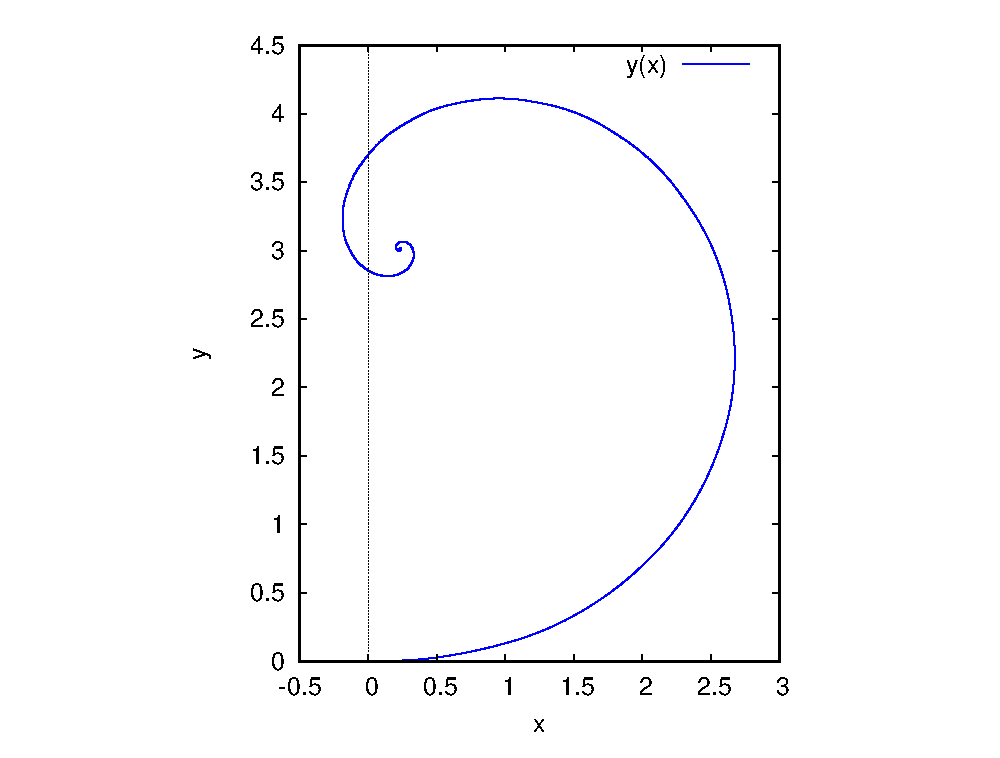
\includegraphics[width=\linewidth]{content/pic/wrench_1000/traj.eps}
                \vspace{-15pt}
                \caption{Траектория}
            \column{0.33\textwidth}
                \centering
                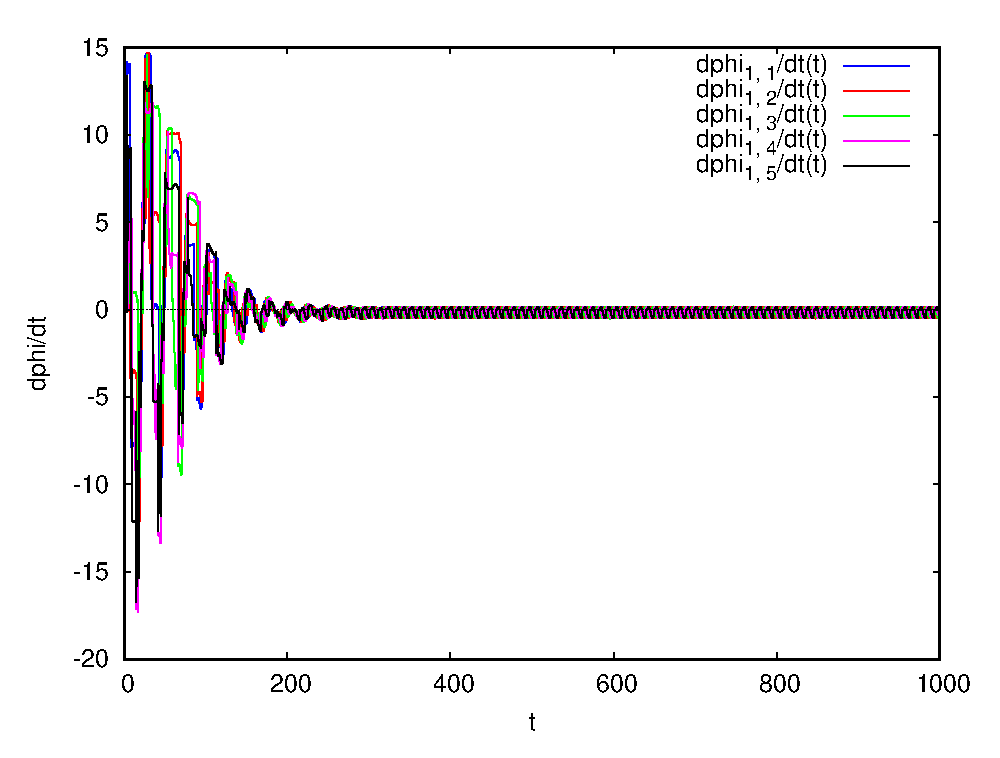
\includegraphics[width=\linewidth]{content/pic/wrench_1000/nus1.eps}
                \vspace{-15pt}
                \caption{$\dot{\mathbf{\phi}}$ на первом колесе}
            \column{0.33\textwidth}
                \centering
                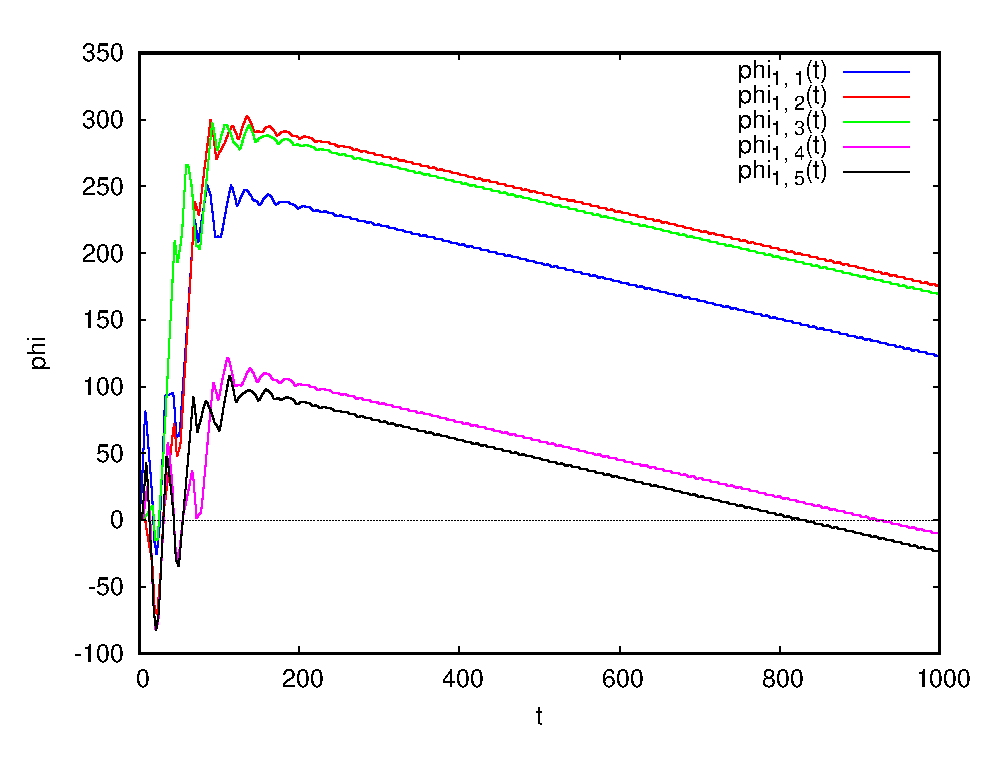
\includegraphics[width=\linewidth]{content/pic/wrench_1000/phi1.eps}
                \vspace{-15pt}
                \caption{углы$\mathbf{\phi}$ на первом колесе}
        \end{columns}
    \end{figure}
\end{frame}

\section{3. Динамика экипажа с трением}

\subsection{Построение и верификация модели}

\begin{frame}{Динамика отдельного ролика}
    \begin{figure}[htb]
        \centering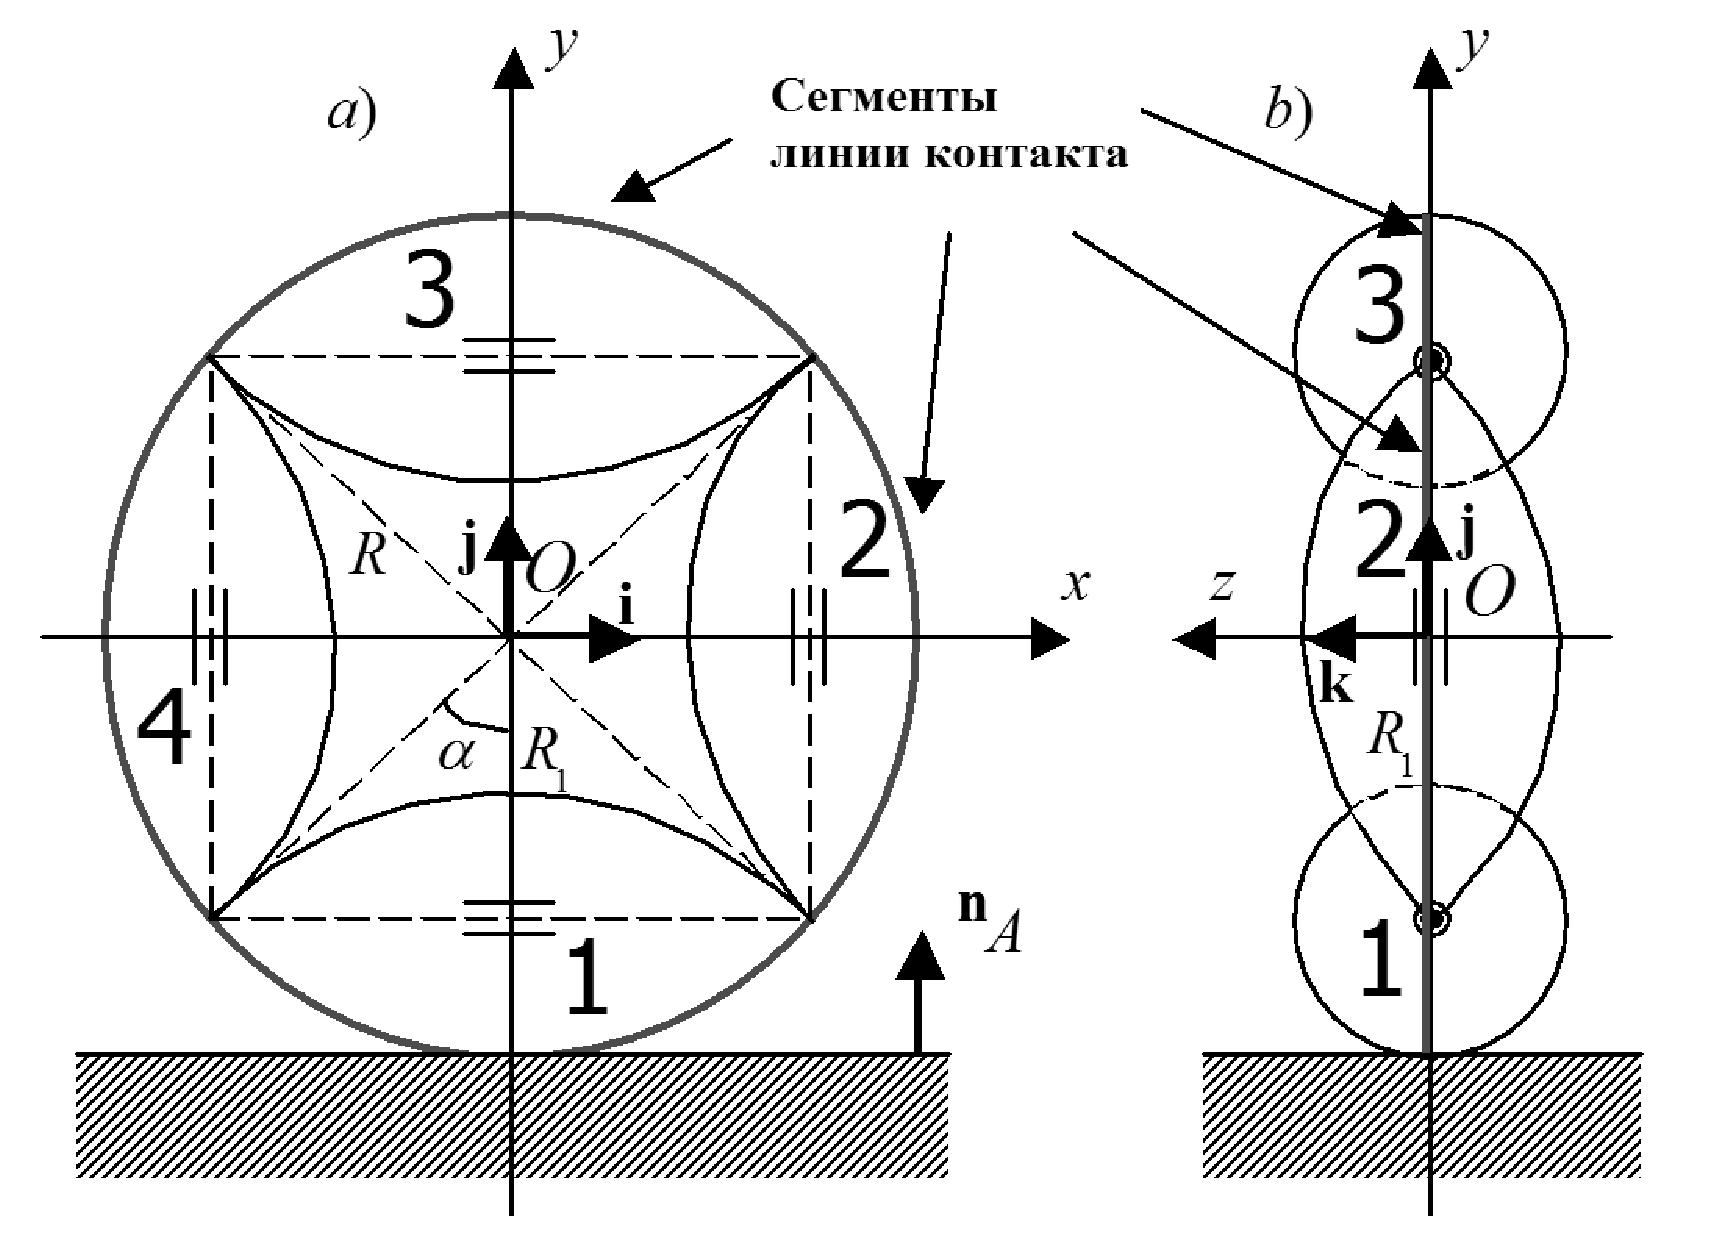
\includegraphics[width=0.65\textwidth]{content/parts/3_friction/nd/OmniWheel.eps}
        \caption{Омни-колесо в вертикальном положении: a) вид сбоку; b) вид спереди.}
    \end{figure}
    $$ x^2+\left(\sqrt{y^2+z^2}+R_1\right)^2=R^2 $$
\end{frame}

\begin{frame}{Отслеживание контакта}
    \minipage{0.5\textwidth}
        \begin{figure}[htb]
            \centering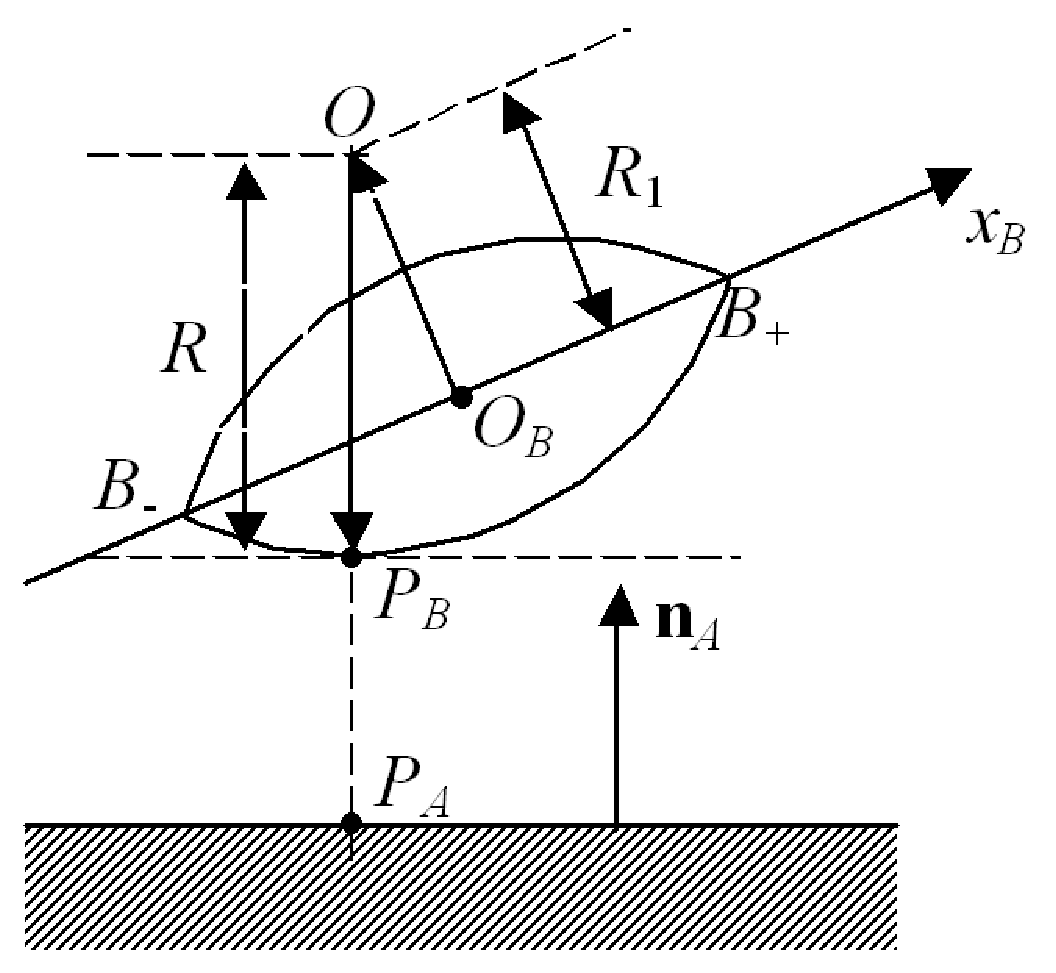
\includegraphics[width=\textwidth]{content/parts/3_friction/nd/RollerSection.eps}
            \caption{Схема отслеживания контакта: вид сбоку отдельного ролика.}
            \label{ContactScheme}
        \end{figure}
    \endminipage
    \minipage{0.5\textwidth}
        $$ {\bf d}=\dfrac{T_B{\bf i}_B\times {\bf n}_A}{\left| T_B{\bf i}_B\times {\bf n}_A\right|} $$
        $$ \overrightarrow{O_BO}=R_1{\bf d}\times T_B{\bf i}_B $$
        $$ {\bf r}_{P_B}={\bf r}_B+R_1{\bf d}\times T_B{\bf i}_B-R{\bf n}_A $$
        $$ {\bf r}_{P_A}=\left( x_{P_B},0,z_{P_B}\right) ^T $$
        $$ \left| T_B{\bf i}_B\cdot {\bf n}_A\right|\le\sin\alpha $$
        $$ y_B<R, \quad y_{P_B}=0, \quad F_n=0 $$
    \endminipage
\end{frame}

\begin{frame}{Структура динамической модели}
    \begin{itemize}
        \item сухое трение, регуляризованное в окрестности $\mathbf{v} = 0$ линейной функцией насыщения
        \item твердое тело платформы, 3 твердых тела колес, 12 твердых тел роликов
        \item для каждого твердого тела 6 ОДУ Ньютона для ц.м. и 7 ОДУ Эйлера (4 кин.ур. для кватерниона и 3 дин.ур. для $\mathbf{\omega}$)
        \item всего $208$ ОДУ плюс дополнительные дифференциальные уравнения, задаваемые связями
    \end{itemize}
\end{frame}

\begin{frame}{Верификация}{Модель для сравнения}
    \begin{figure}[H]
        \centering
        \begin{columns}
            \column{0.45\textwidth}
                \centering
                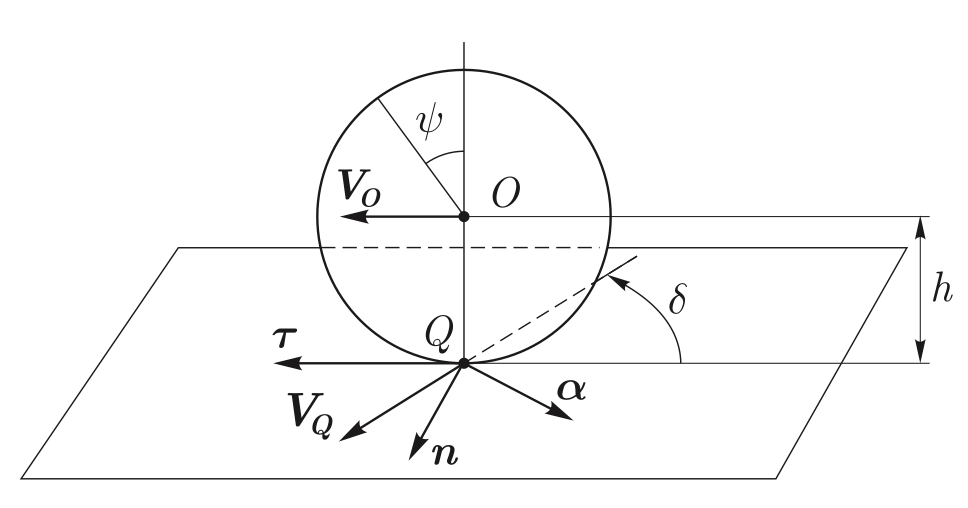
\includegraphics[width=\textwidth]{content/parts/3_friction/diploma/img/art/bor_wheel_scheme.png}
                \caption{Модель колеса}
                \label{fig:bor_wheel_scheme}
            \column{0.45\textwidth}
                \centering
                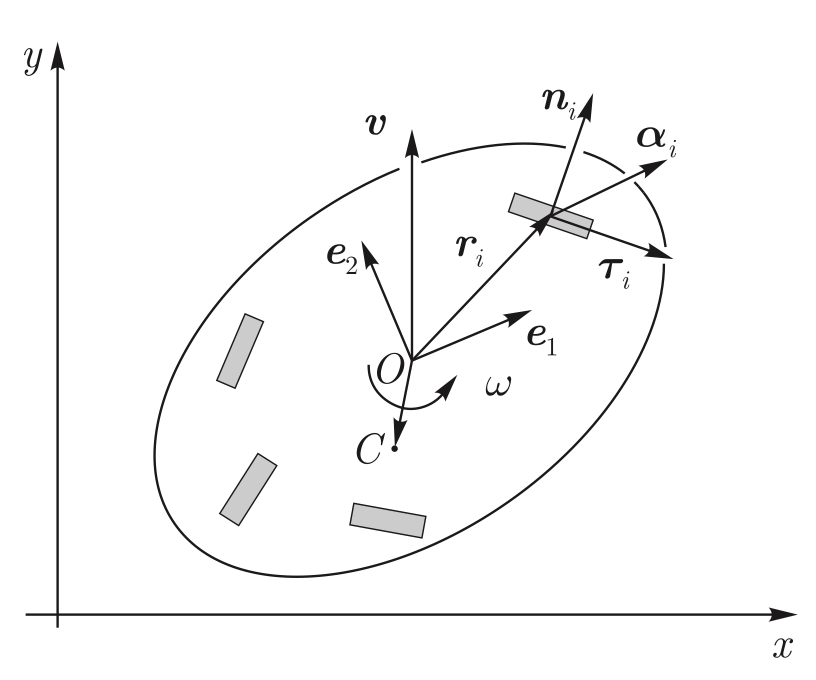
\includegraphics[width=\textwidth]{content/parts/3_friction/diploma/img/art/bor_vehicle.png}
                \caption{Модель экипажа}
                \label{fig:bor_vehicle}
        \end{columns}
    \end{figure}
\end{frame}

\begin{frame}{Верификация}{Варианты движений}
    \begin{figure}[!ht]
        \centering
        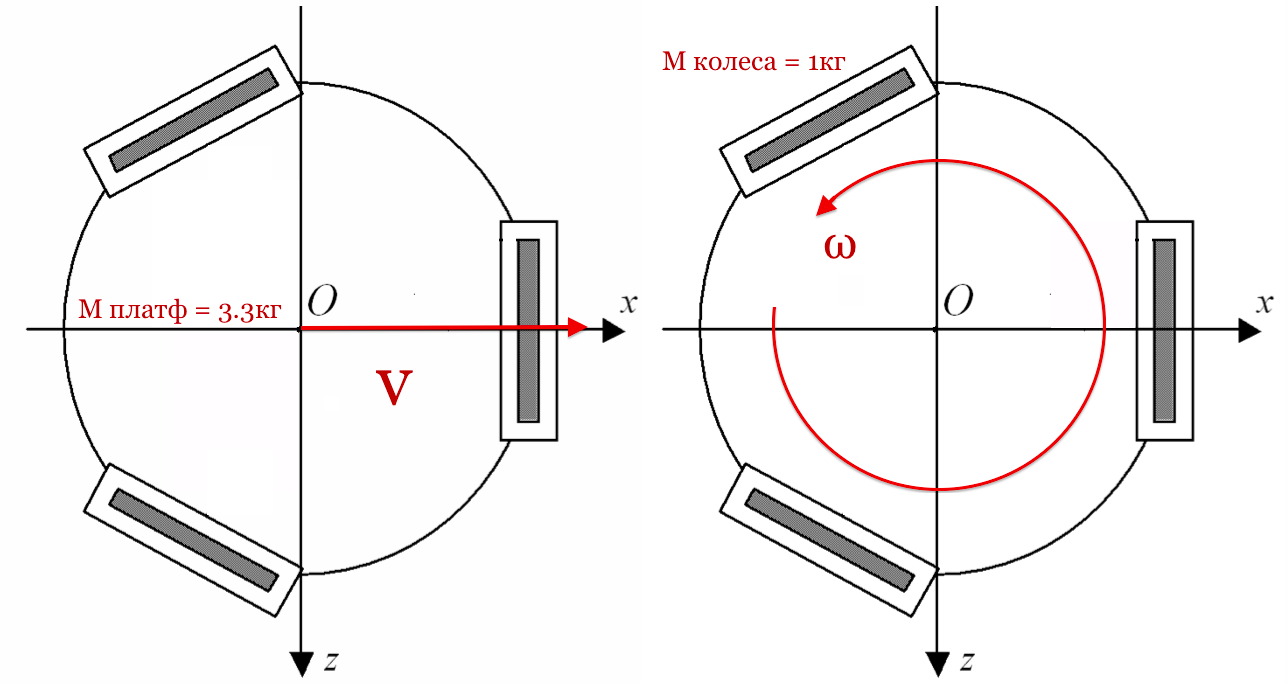
\includegraphics[width=0.95\textwidth]{content/parts/3_friction/diploma/img/art/my_exp_setup.png}
        \caption{Параметры экспериментов}
        \label{fig:my_exp_setup}
    \end{figure}
    испытания -- при $\sum m_{\text{рол}} \rightarrow 0$
\end{frame}

\begin{frame}{Верификация -- Вращение вокруг вертикальной оси}
    \vspace{-50pt}
    \begin{figure}[h]
        \begin{center}\begin{equation*}\begin{array}{cc}
            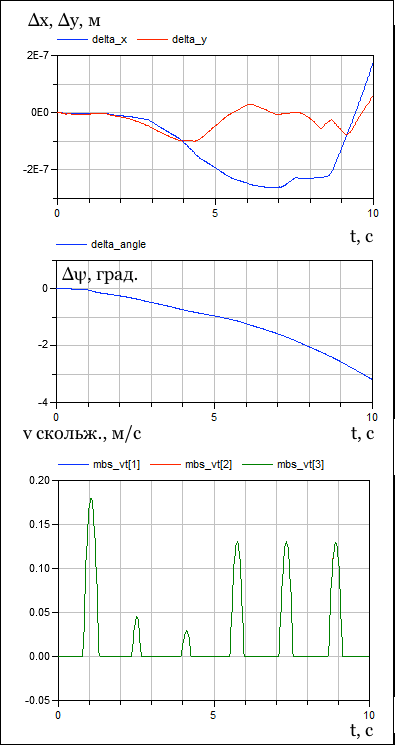
\includegraphics[width=0.4\textwidth, viewport=0 0 395 745,clip]{content/parts/3_friction/diploma/img/res/comparison_v_0_0_omega_1_frac_1e-1_n_4_time_10s.png} 
            &
            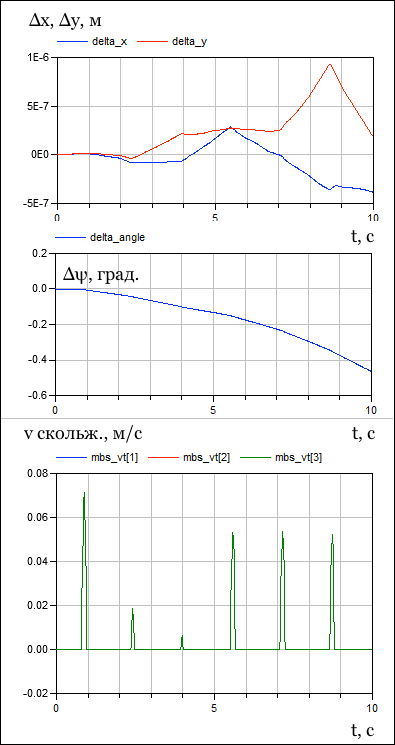
\includegraphics[width=0.4\textwidth, viewport=0 0 395 745,clip]{content/parts/3_friction/diploma/img/res/comparison_v_0_0_omega_1_frac_1e-2_n_4_time_10s.png}\\
            \eta = 10^{-5}, v_0 = 0, \omega_0 = 1 & \eta = 10^{-6}, v_0 = 0, \omega_0 = 1\\
        \end{array}\end{equation*}\end{center}
        \caption{Вращение экипажа с трением вокруг вертикальной оси}
    \end{figure}
\end{frame}

\begin{frame}{Верификация -- Вращение вокруг вертикальной оси}
    \vspace{-50pt}
    \begin{figure}[h]
        \begin{center}\begin{equation*}\begin{array}{cc}
            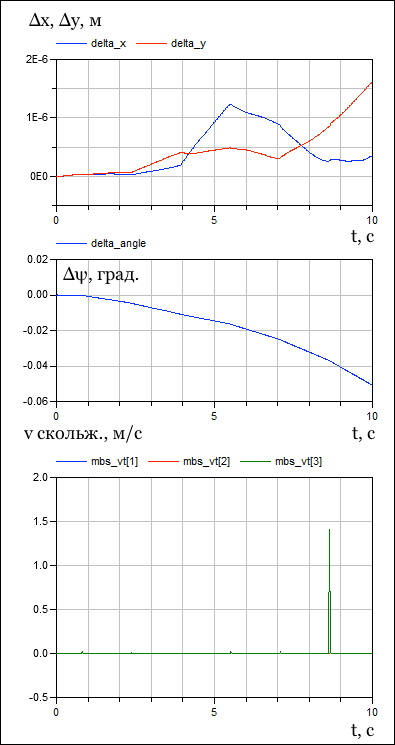
\includegraphics[width=0.4\textwidth, viewport=0 0 395 745,clip]{content/parts/3_friction/diploma/img/res/comparison_v_0_0_omega_1_frac_1e-3_n_4_time_10s.png} 
            &
            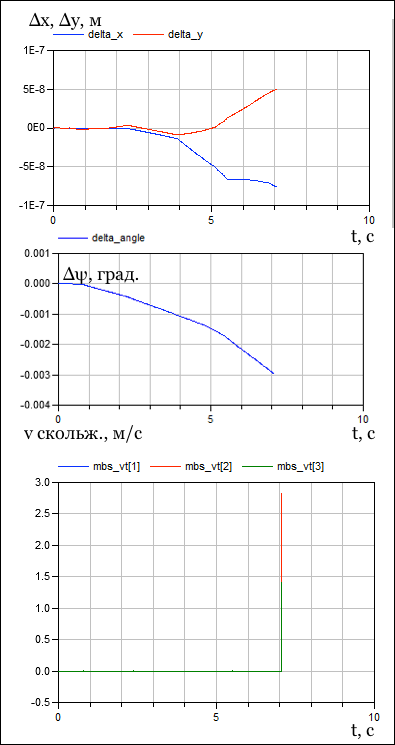
\includegraphics[width=0.4\textwidth, viewport=0 0 395 745,clip]{content/parts/3_friction/diploma/img/res/comparison_v_0_0_omega_1_frac_1e-4_n_4_time_10s.png}\\
            \eta = 10^{-5}, v_0 = 0, \omega_0 = 1 & \eta = 10^{-6}, v_0 = 0, \omega_0 = 1\\
        \end{array}\end{equation*}\end{center}
        \caption{Вращение экипажа с трением вокруг вертикальной оси}
    \end{figure}
\end{frame}

\begin{frame}{Верификация -- Вращение вокруг вертикальной оси}
    \vspace{-50pt}
    \begin{figure}[h]
        \begin{center}\begin{equation*}\begin{array}{cc}
            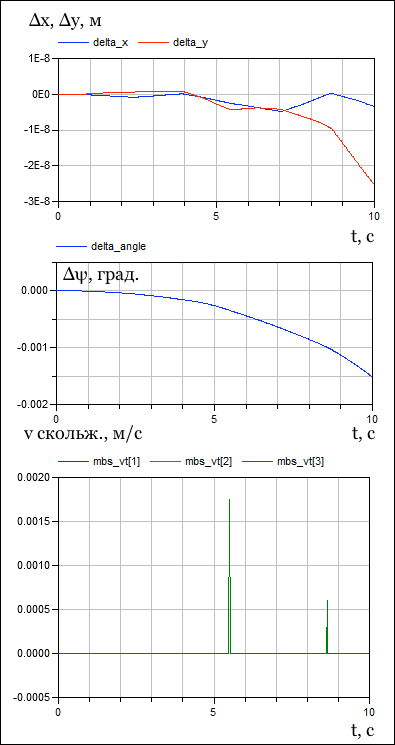
\includegraphics[width=0.4\textwidth, viewport=0 0 395 745,clip]{content/parts/3_friction/diploma/img/res/comparison_v_0_0_omega_1_frac_1e-5_n_4_time_10s.png} 
            &
            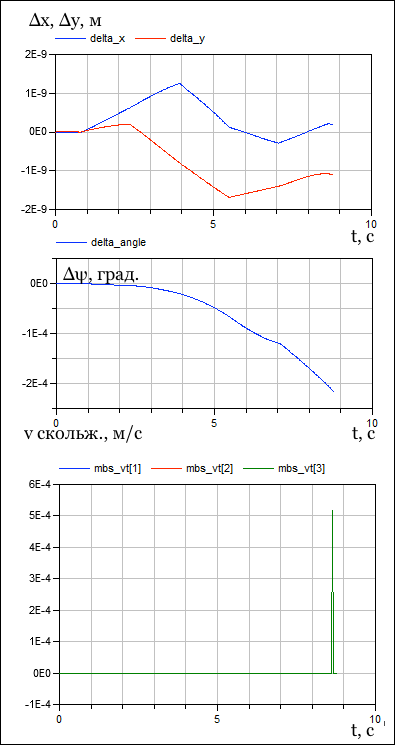
\includegraphics[width=0.4\textwidth, viewport=0 0 395 745,clip]{content/parts/3_friction/diploma/img/res/comparison_v_0_0_omega_1_frac_1e-6_n_4_time_10s.png}\\
            \eta = 10^{-5}, v_0 = 0, \omega_0 = 1 & \eta = 10^{-6}, v_0 = 0, \omega_0 = 1\\
        \end{array}\end{equation*}\end{center}
        \caption{Вращение экипажа с трением вокруг вертикальной оси}
    \end{figure}
\end{frame}

\begin{frame}{Верификация -- Движение по прямой}
    \vspace{-50pt}
    \begin{figure}[h]
        \begin{center}\begin{equation*}\begin{array}{cc}
            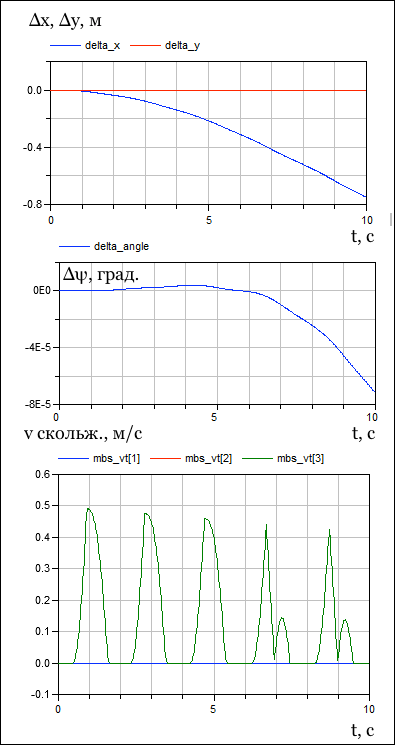
\includegraphics[width=0.4\textwidth, viewport=0 0 395 745,clip]{content/parts/3_friction/diploma/img/res/comparison_v_1_0_omega_0_frac_1e-1_n_4_time_10s.png}
            &
            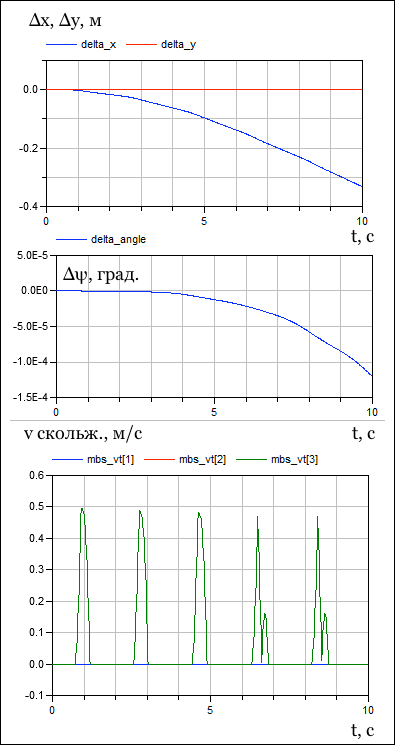
\includegraphics[width=0.4\textwidth, viewport=0 0 395 745,clip]{content/parts/3_friction/diploma/img/res/comparison_v_1_0_omega_0_frac_1e-2_n_4_time_10s.png}\\
            \eta = 0,001, v_0 = 1, \omega_0 = 0 & \eta = 0,0001, v_0 = 1, \omega_0 = 0\\
        \end{array}\end{equation*}\end{center}
        \caption{Вращение экипажа с трением по прямой}
    \end{figure}
\end{frame}

\begin{frame}{Верификация -- Движение по прямой}
    \vspace{-50pt}
    \begin{figure}[h]
        \begin{center}\begin{equation*}\begin{array}{cc}
            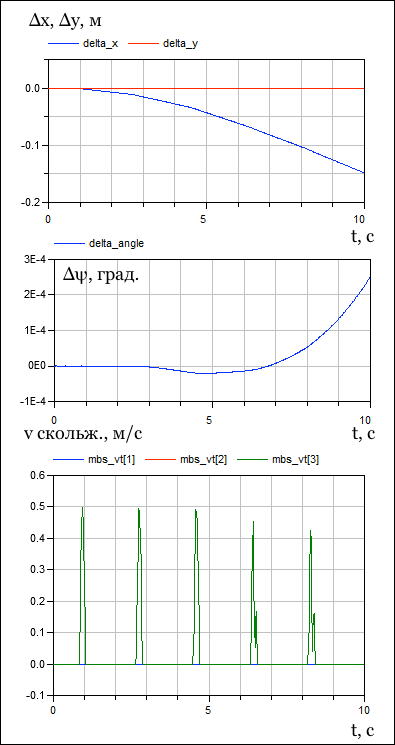
\includegraphics[width=0.4\textwidth, viewport=0 0 395 745,clip]{content/parts/3_friction/diploma/img/res/comparison_v_1_0_omega_0_frac_1e-3_n_4_time_10s.png}
            &
            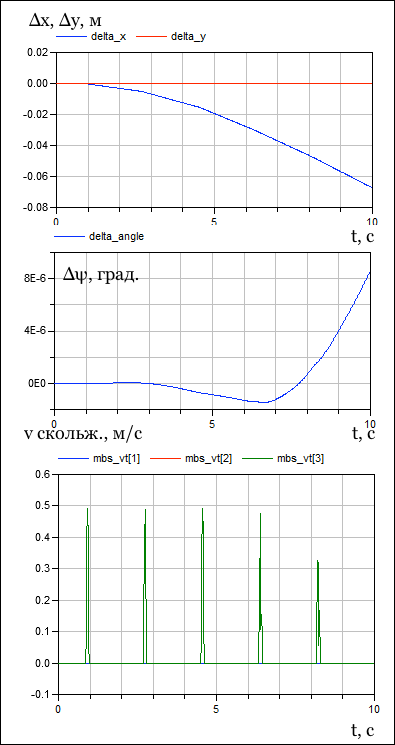
\includegraphics[width=0.4\textwidth, viewport=0 0 395 745,clip]{content/parts/3_friction/diploma/img/res/comparison_v_1_0_omega_0_frac_1e-4_n_4_time_10s.png}\\
            \eta = 0,001, v_0 = 1, \omega_0 = 0 & \eta = 0,0001, v_0 = 1, \omega_0 = 0\\
        \end{array}\end{equation*}\end{center}
        \caption{Вращение экипажа с трением по прямой}
    \end{figure}
\end{frame}

\begin{frame}{Результаты}
    \begin{enumerate}
        \item Получены уравнения движения экипажа на омни-колесах по абс. шероховатой плоскости с учетом инерции роликов
        \item Изучены их свойства и проведено сравнение с уравнениями движения безынерционной модели
        \item Построен способ расчета изменения обобщенных скоростей при смене ролика в контакте с точки зрения теории удара
        \item Получены численные решения для симметричной конфигурации экипажа
        \item Построена динамическая модель на плоскости с регуляризованным сухим трением
        \item Выполнена верификация динамической с использованием безынерционной модели
    \end{enumerate}
    \vspace{-10pt}
    \centering
    \textcolor{Periwinkle}{Спасибо за внимание!}
\end{frame}

\bibliography{content/omni}   % name your BibTeX data base

\end{document}


